\section{Gut microbiota transfer and the turquoise killifish mucosal repertoire}
\label{sec:igseq_gut}

\newabbreviation{bellemans}{GRZ-Bellemans}{Substrain of GRZ}

The results from \Cref{sec:igseq_ageing} demonstrate that the whole-body antibody repertoire of adult male turquoise killifish declines in % (clonal)
alpha-diversity with age, while increasing in VJ beta-diversity. % TODO: ... other summarised results go here
These results suggest that ... . % TODO: Finish summary

However, while these results demonstrate significant age-related changes in repertoire composition at the level of the entire body, they give no specific information about the ageing process exhibited by the specialised repertoires of particular immune organs, which could differ substantially as a result of their distict antigenic environments and B-cell-subpopulation composition (\Cref{sec:intro_immunosenescence}). In particular, the gut mucosal repertoire, which polices the interface between the host organism and the gut microbiota, represents a highly important B-cell subpopulation with an intense and distinctive exprience of antigenic exposure. % TODO: Citation needed
It would therefore be interesting to learn whether the pattern of repertoire ageing observed in the gut accords with that seen in the wider body, or exhibits its own distinct ageing phenotypes.

Smith \textit{et al.} \parencite{smith2017microbiota} demonstrated that gut microbiota transfer from young to middle-aged turquoise killifish significantly extends lifespan in this species, as well as significantly altering microbiota composition and gene expression in the gut. As part of these experiments, gut total RNA was collected from a number of male turquoise killifish of the GRZ-Bellemans substrain (a closely-related substrain to the GRZ-AD substrain used in \Cref{sec:igseq_ageing}) at different ages and following different experimental interventions (\Cref{fig:igseq-gut-design,tab:gut-cohorts-summary,tab:gut-cohorts-fish}). By using these RNA samples to perform a further round of \Igseq in the turquoise killifish, I hoped to investigate the effects of both age and microbiota transfer on the diversity of the gut mucosal repertoire; in particular, given the observed lifespan effect of gut-microbiota transfer and the intimate relationship between the gut microbiota and the mucosal adaptive immune system, % TODO: Citation needed
I hypothesised that gut microbiotal transfer might significantly ameliorate the ageing of the adaptive-immune repertoire seen in \Cref{sec:igseq_ageing}, either through delaying the decline in diversity observed in older fish or by stimulating a renewal of repertoire diversity in mucosal B-cells.

\begin{figure}
\centering
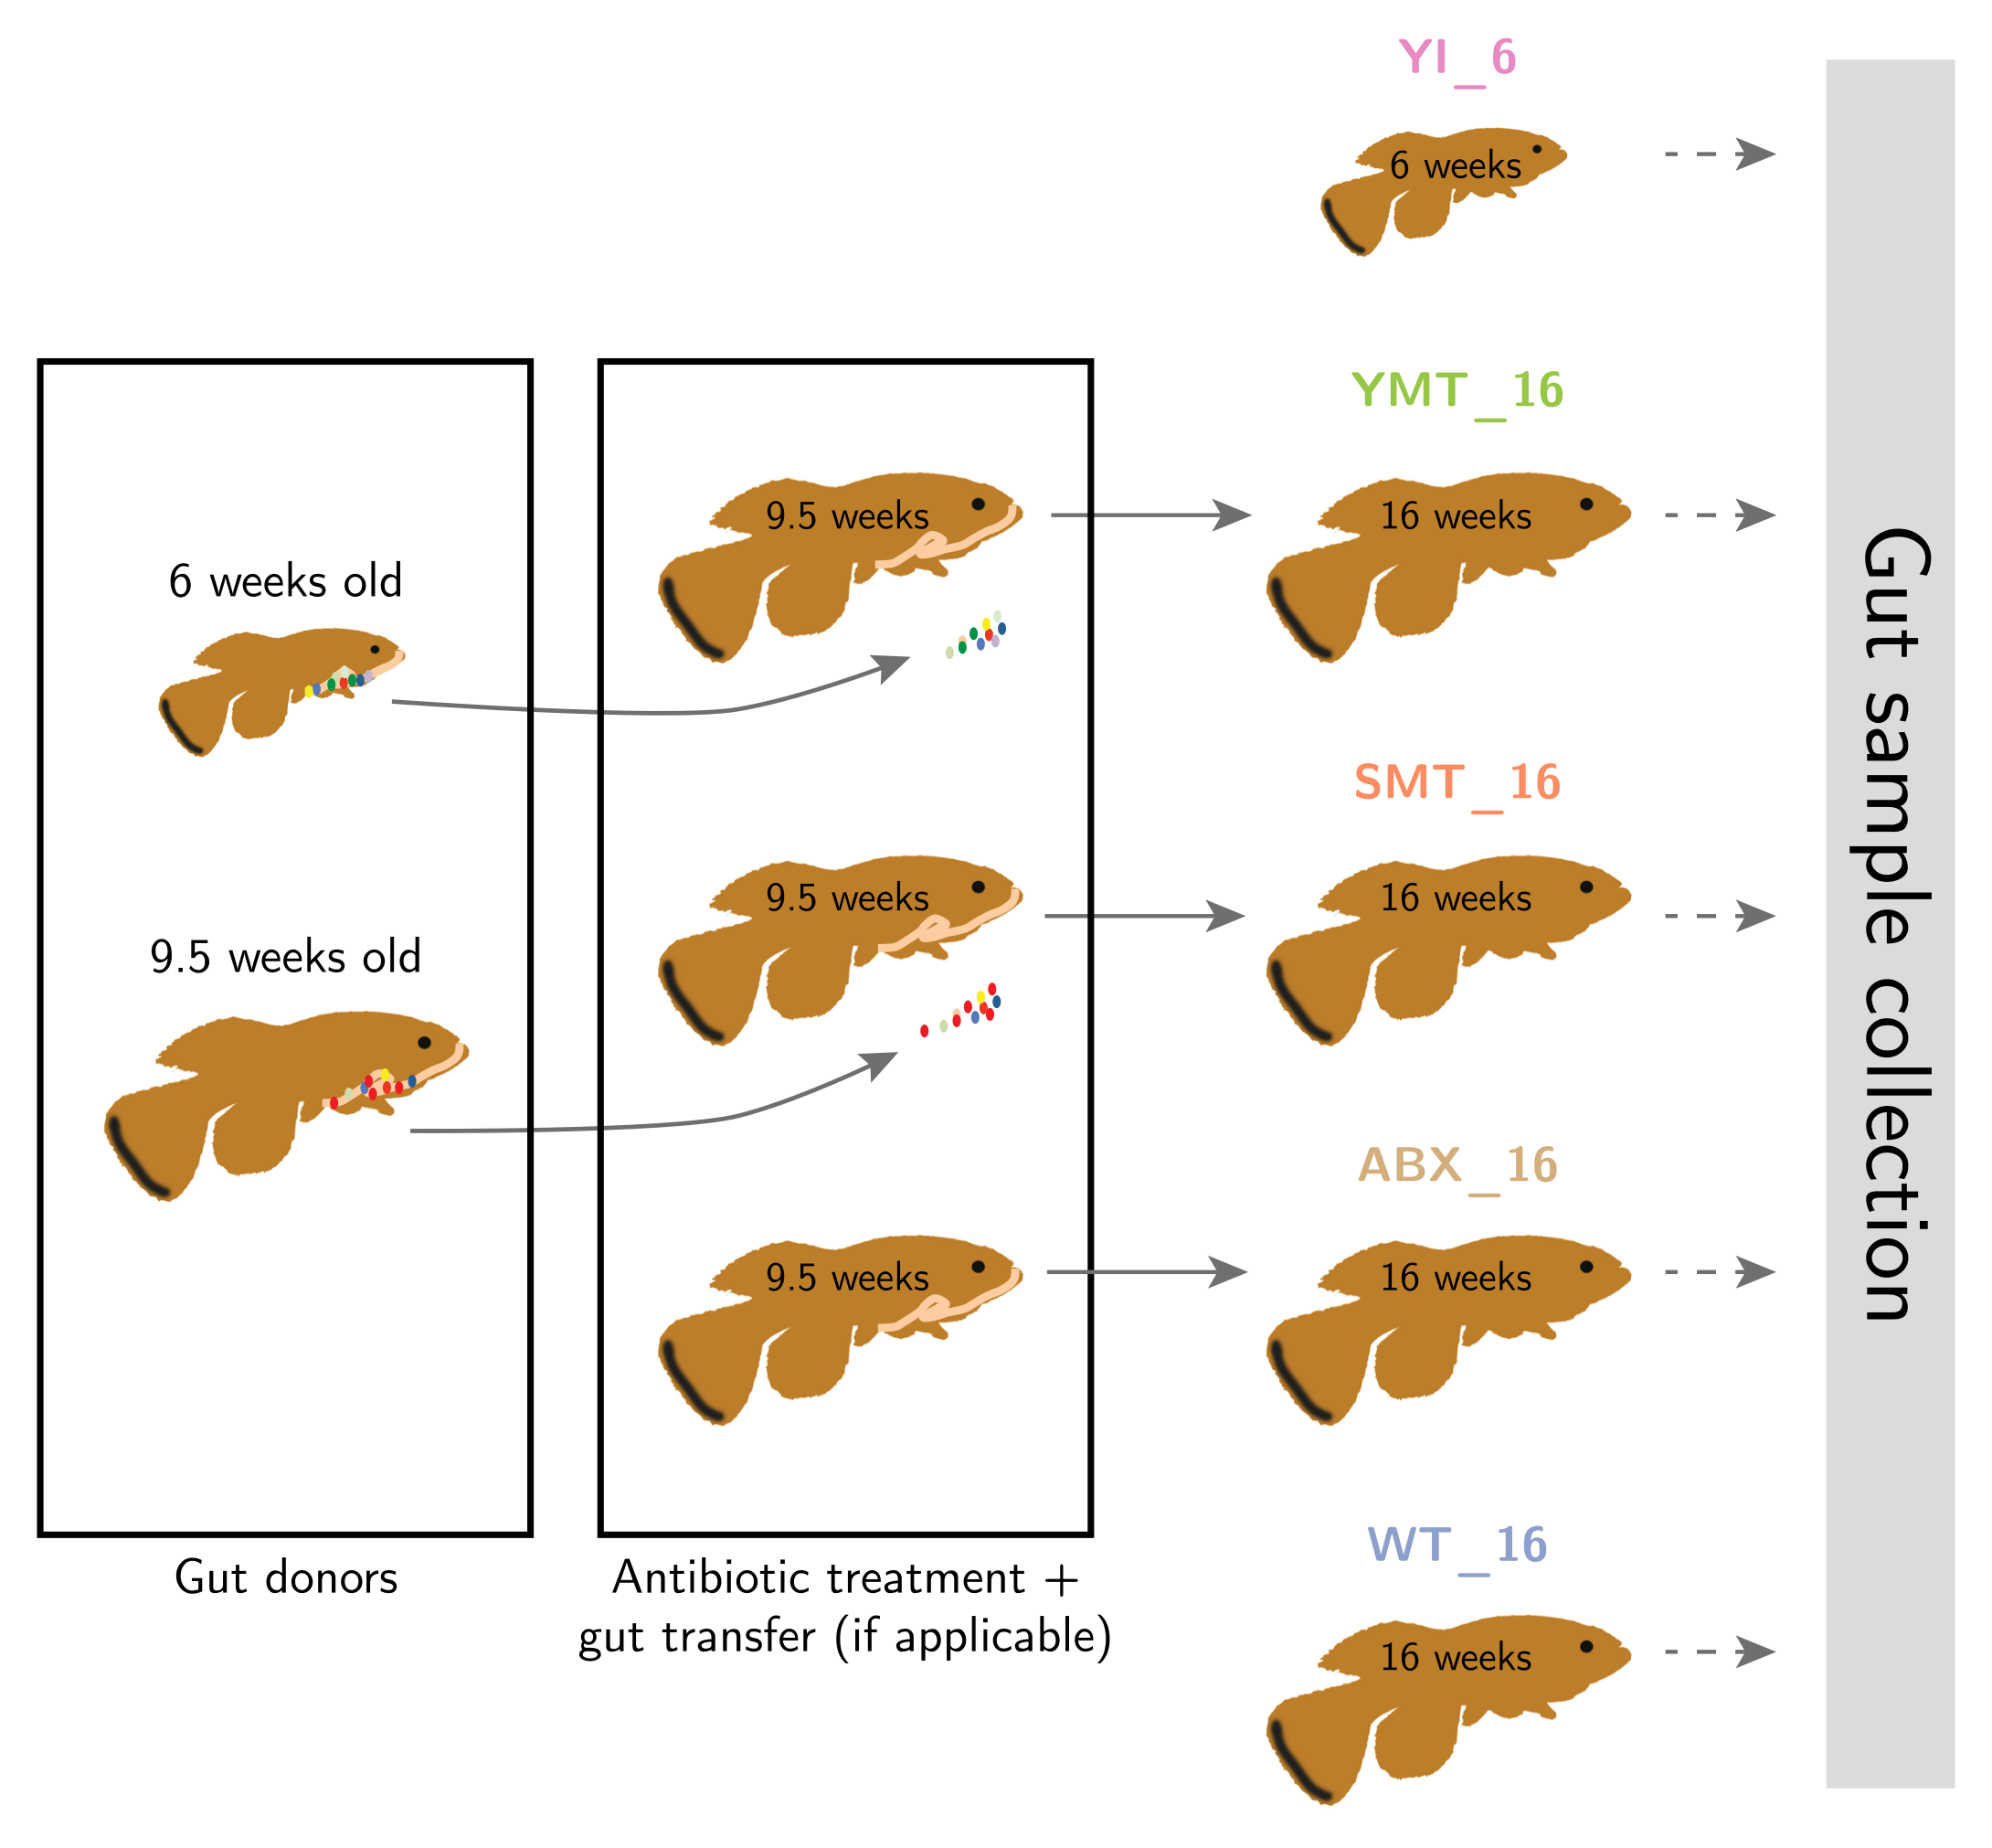
\includegraphics[width = 0.8\textwidth]{_Figures/png_edited/gut-design}
\caption[Experimental design of killifish gut-microbiota transfer study]{\textbf{Experimental design of killifish \gut-microbiota transfer study}: Schematic of the design of the gut-microbiota transfer experiment in Smith \textit{et al.} \parencite{smith2017microbiota}. Groups YI\_6 and WT\_16 were sacrificed without experimental intervention at 6 and 16 weeks, respectively, while the others recieved antibiotic treatment at 9.5 weeks followed by either no further intervention (ABX\_16) or gut-microbiota transfer from a 6-week-old (YMT\_16) or 9.5-week-old (SMT\_16) donor. Adapted from \parencite{smith2017microbiota}, Figure 4.}
\label{fig:igseq-gut-design}
\end{figure}

\begin{table}[b]
\centering
% latex table generated in R 3.5.2 by xtable 1.8-3 package
% Mon Mar 11 16:51:04 2019
\begin{tabular}{lrlll}
  \toprule Group & Age (weeks) & \# Fish (Sequenced/Total) & Antibiotics? & Microbiota Transfer? \\ 
  \midrule YI\_6 & 6 & 4 / 4 & No & No \\ 
  WT\_16 & 16 & 3 / 4 & No & No \\ 
  ABX\_16 & 16 & 4 / 4 & Yes & No \\ 
  SMT\_16 & 16 & 3 / 4 & Yes & Yes (9.5-week-old donor) \\ 
  YMT\_16 & 16 & 4 / 4 & Yes & Yes (6-week-old donor) \\ 
   \bottomrule \end{tabular}

\caption{Summary of killifish used in \igseq validation and ageing experiment. All fish are GRZ-Bellemans strain and male.}
\label{tab:gut-cohorts-summary}
\end{table}

Of the twenty samples outlined in \Cref{tab:gut-cohorts-summary,tab:gut-cohorts-fish}, one (fish 400, from the WT\_16wk group) contained too little RNA to undergo \igseq library preparation, while another (fish 1005, from the OMT\_16wk group) was too degraded for a useful library to be obtained. The remaining 18 samples underwent \igseq library preparation, performed by Aleksandra Placzek and Michael Poeschla using the protocol I designed in \Cref{sec:igseq_protocol_library}. Several of the other samples were also somewhat degraded, with RNA integrity numbers between 5.5 and 7.0 (\Cref{tab:gut-cohorts-fish}), but succeeded in producing useable libraries; these samples were included in the sequencing pool, but the RIN values from each sample were retained for comparison with downstream quality-control measures following \Igseq. The resulting libraries were sequenced together in two MiSeq runs, yielding a total of \embed{_Figures/txt/ageing-reads-raw-total.txt} million read pairs (\embed{_Figures/txt/gut-reads-raw-min.txt} to \embed{_Figures/txt/gut-reads-raw-max.txt} million pairs per individual), and the resulting reads underwent pre-processing, filtering and clonotyping as described in \Cref{sec:igseq_pilot,sec:igseq_ageing}.

Compared to the datasets in those sections, the gut dataset exhibited highly consistent behaviour up to and including VDJ assignment and Change-O database construction, with \embed{_Figures/txt/gut-read-survival-init-min.txt}\,\% to \embed{_Figures/txt/gut-read-survival-init-max.txt}\,\% of reads surviving up to this stage in the pipeline (\Cref{fig:igseq-gut-read-survival-all}). However, a substantially higher proportion of reads (\embed{_Figures/txt/gut-read-survival-rel-loss-total.txt}\,\%) are lost during V-score filtering (\Cref{fig:igseq-gut-functional-prop}) and clonotyping, with some individuals losing as much as \embed{_Figures/txt/gut-read-survival-rel-loss-max.txt}\,\% of their input reads during these stages. The amount of reads lost at this stage did not appear to have any relationship with the RNA integrity of the samples (\Cref{fig:igseq-gut-read-survival-all-rin}, $r \approx -0.1$, $p \approx 0.7$), and following V-score filtering the functional composition of surviving sequences was similar to that of the other datasets (\Cref{fig:igseq-gut-functional-prop-post,fig:igseq-ageing-functional-prop-post,fig:igseq-pilot-functional-prop-b}). Nevertheless, to avoid any problems associated with very low numbers (and possibly low quality) of input reads, individuals with fewer than 30\% of input reads surviving through filtering and clonotyping were excluded from downstream analysis; two individuals (1274 and 1309, both from the antibotics-treated group) were excluded in this way (\Cref{fig:igseq-gut-read-survival-all-rel}).

\begin{figure}
\centering
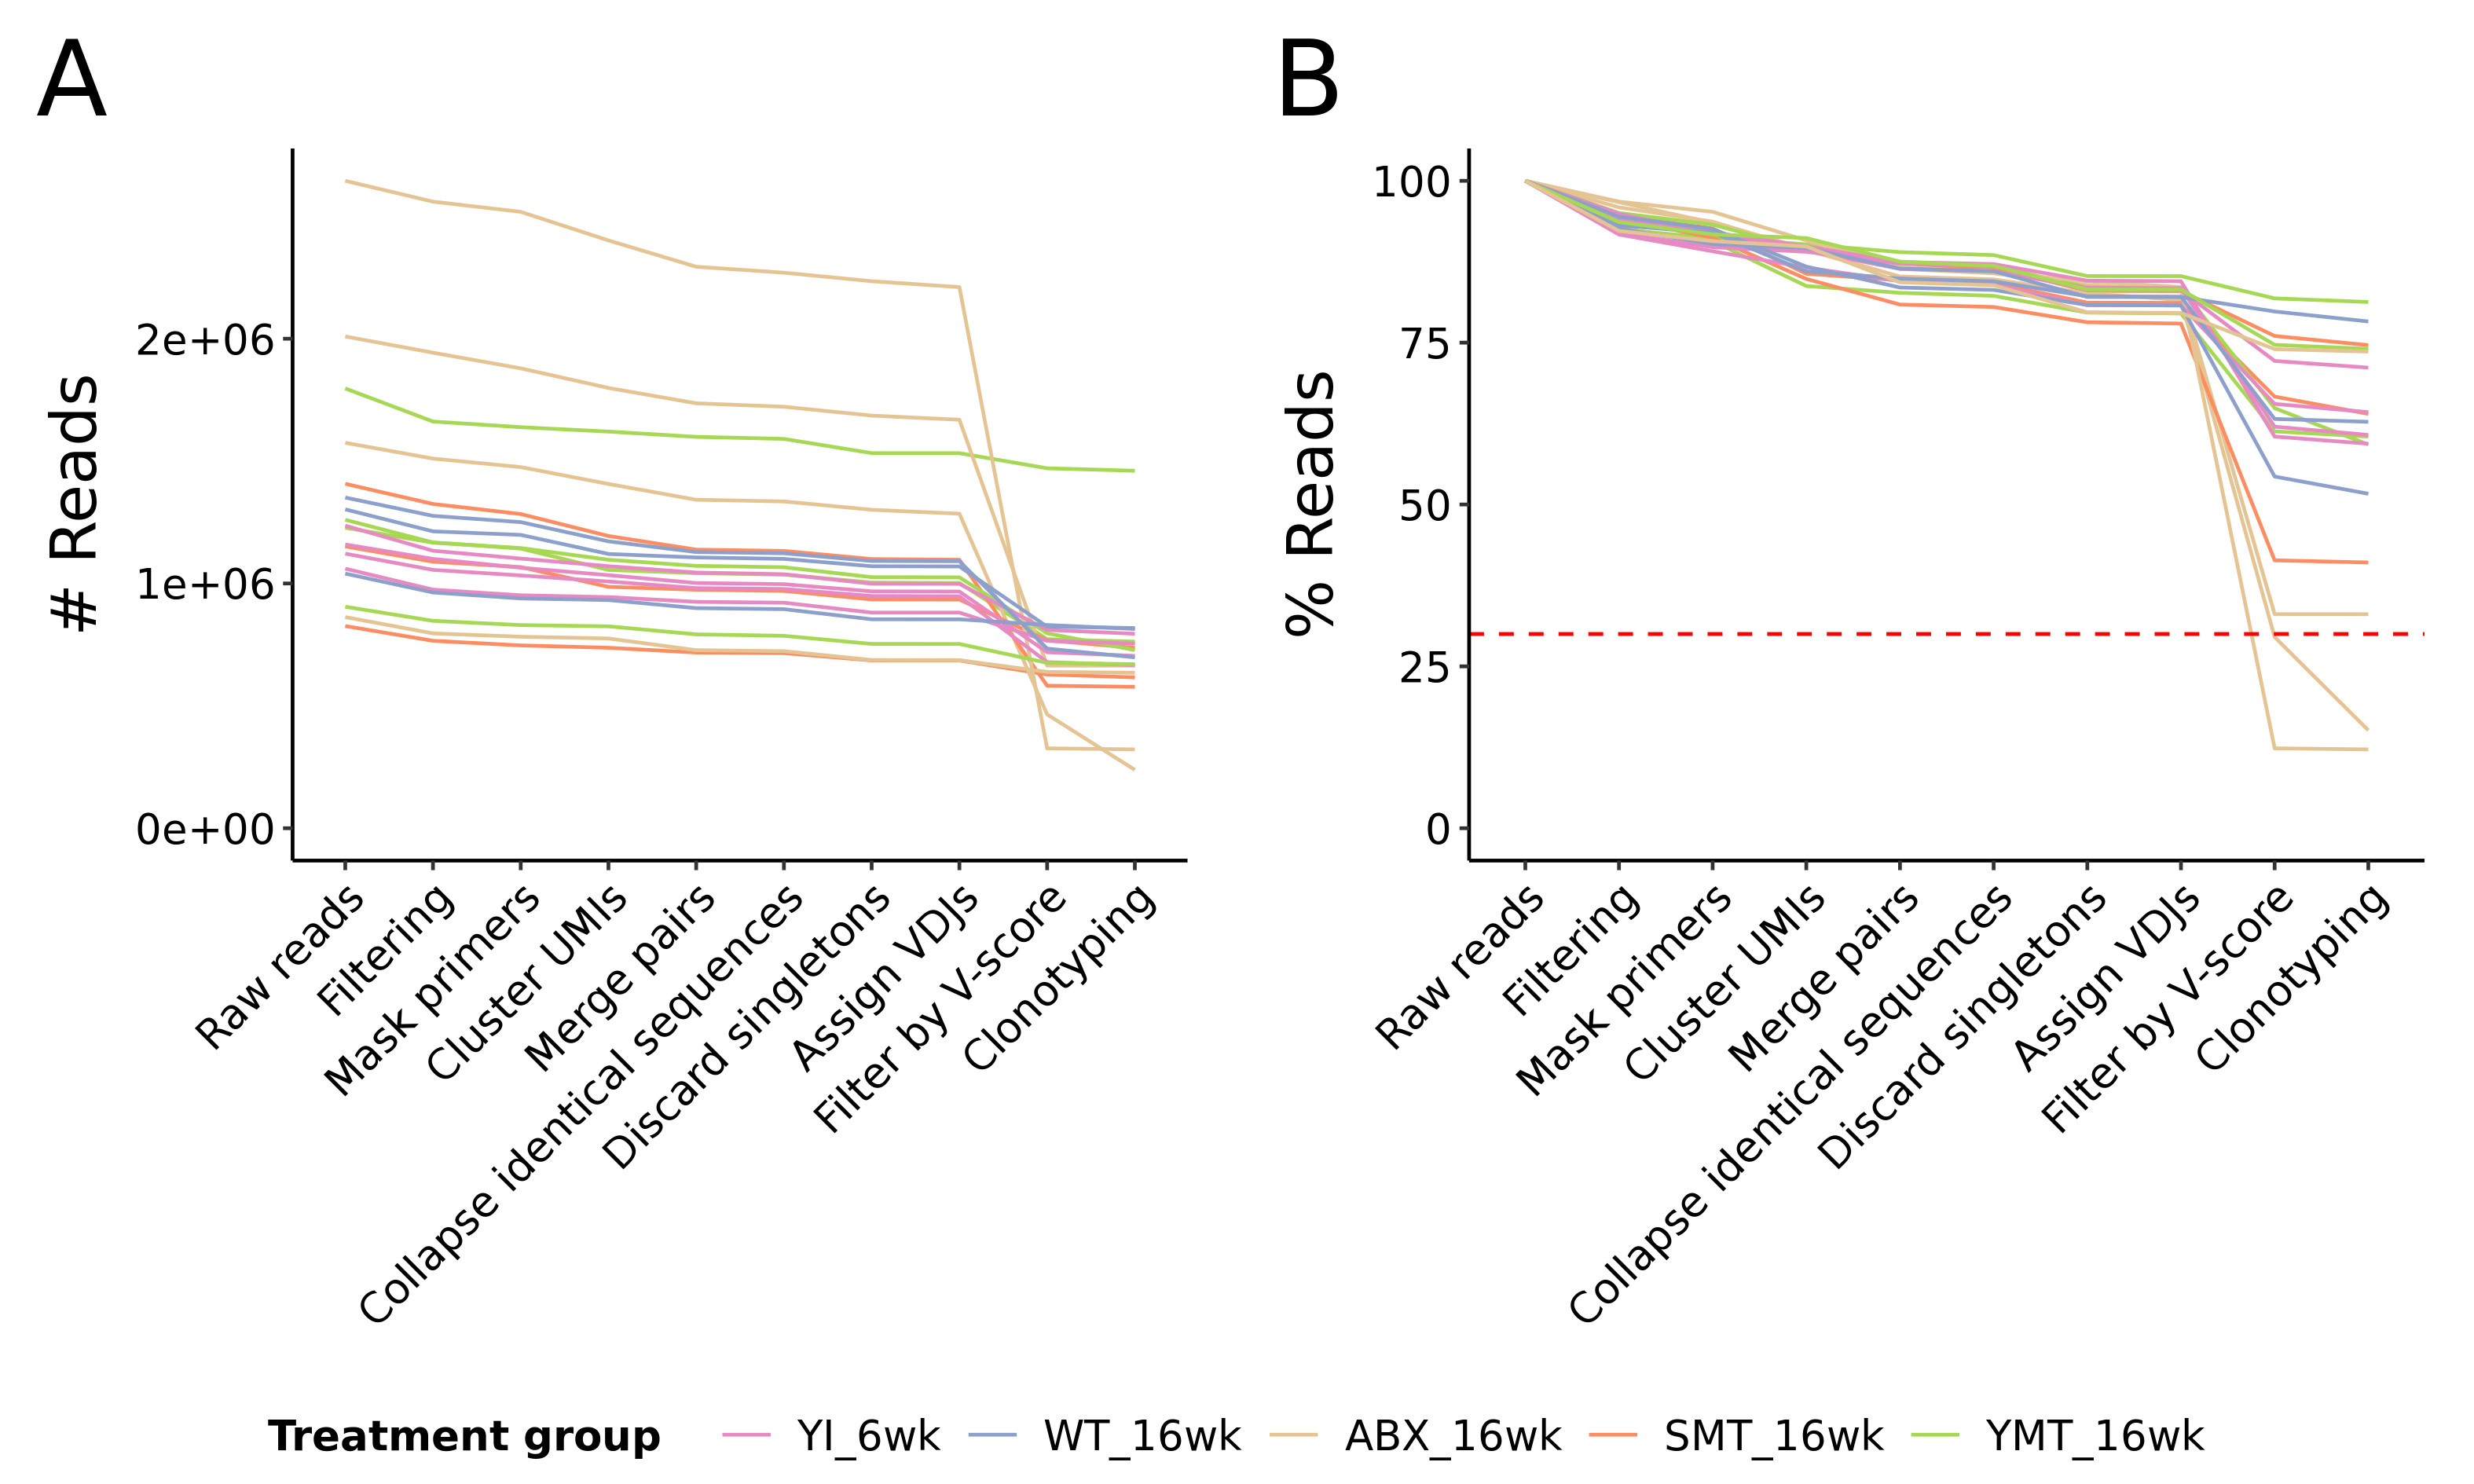
\includegraphics[width = 0.9\textwidth]{_Figures/png/gut-read-survival-all.png}
\begin{subfigure}{0em}
\phantomsubcaption{}
\label{fig:igseq-gut-read-survival-all-abs}
\end{subfigure}
\begin{subfigure}{0em}
\phantomsubcaption{}
\label{fig:igseq-gut-read-survival-all-rel}
\end{subfigure}
\caption[Read survival during pre-processing of \igseq gut dataset]{\textbf{Read survival during pre-processing of \igseq gut dataset:} Line graphs of absolute (A) and relative (B) read survival during pre-processing of the \igseq ageing dataset, up to and including clonotyping. The dotted red line in (B) indicates the 30\% read-survival cutoff, below which samples are discarded prior to downstream analysis.}
\label{fig:igseq-gut-read-survival-all}
\end{figure}

\begin{figure}
\centering
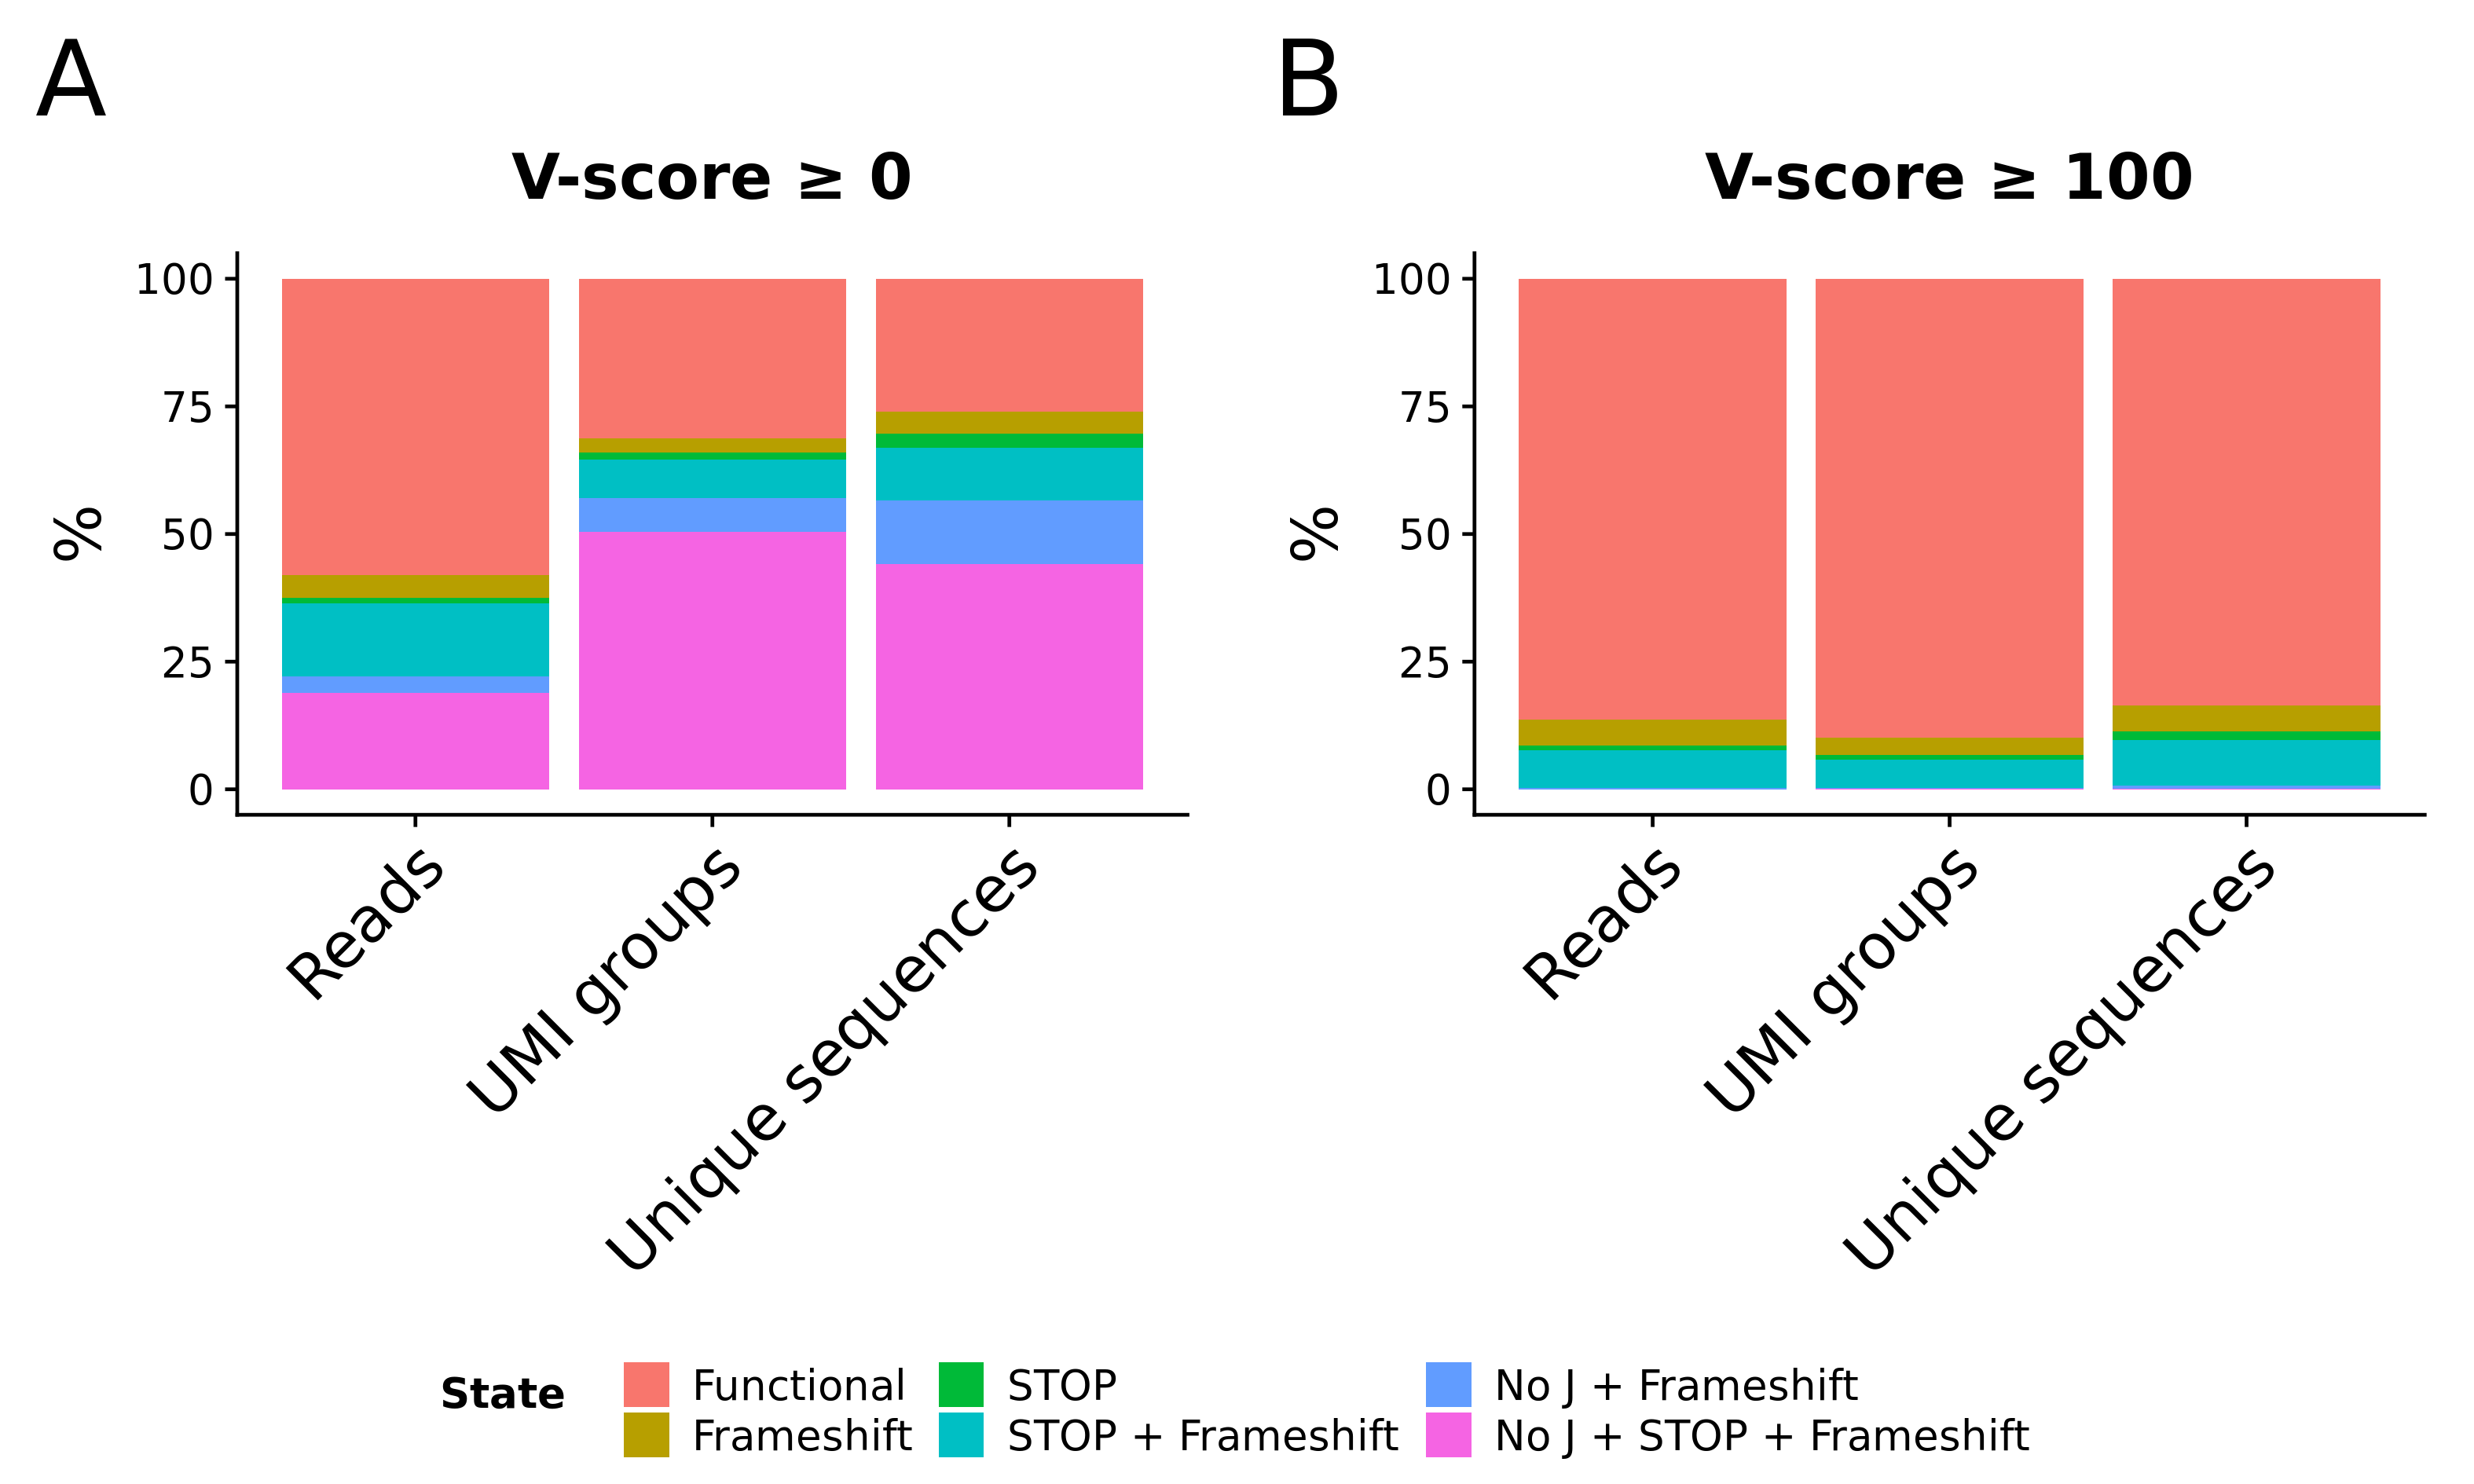
\includegraphics[width = 0.9\textwidth]{_Figures/png/gut-functional-prop}
\begin{subfigure}{0em}
\phantomsubcaption{}
\label{fig:igseq-gut-functional-prop-pre}
\end{subfigure}
\begin{subfigure}{0em}
\phantomsubcaption{}
\label{fig:igseq-gut-functional-prop-post}
\end{subfigure}
\caption[Functional composition and V-score filtering of \igseq ageing dataset]{\textbf{Functional composition and V-score filtering of \igseq ageing dataset:} Proportion of input reads, UMI groups and unique sequences in the \igseq gut-microbiota-transfer dataset belonging to different (non)functional categories, before (A) and after (B) filtering on V-alignment score.}
\label{fig:igseq-gut-functional-prop}
\end{figure}

Following V-score filtering and exclusion of high-read-loss individeals, \embed{_Figures/txt/gut-nseq-assigned-clones.txt}\,\% of remaining unique sequences in the ageing dataset were successfully assigned clonal identities, with the number of clones inferred per individual ranging from \embed{_Figures/txt/igseq-gut-nclones-individual-min.txt} to \embed{_Figures/txt/igseq-gut-nclones-individual-max.txt}, with a median of \embed{_Figures/txt/igseq-gut-nclones-individual-med.txt}; as in the ageing dataset, there is a non-significant (Kruskal-Wallis analysis of variance, $p=\embed{_Figures/txt/igseq-gut-nclones-kruskal-age-p.txt}$) decline in number of clones per individual with age (\Cref{fig:igseq-gut-nclones}). With two exceptions (visible in \Cref{fig:igseq-gut-nclones}), these clonal counts are dramatically lower than those of either the pilot or ageing dataset, both in absolute terms (\Cref{fig:igseq-comparative-metrics-abs}) and relative to the number of UMI groups or unique sequences in each repertoire (\Cref{fig:igseq-comparative-metrics-rel}). This suggests, not entirely surprisingly, that killifish guts contain many fewer B-cell clones than whole-body killifish samples; however, the metrics presented in \Cref{fig:igseq-comparative-metrics} are strongly dependent on the size of each dataset and cannot be taken at face value: for example, even though the pilot dataset contains the same type of sample and even a subset of the same individuals from the ageing dataset, their distributions in \Cref{fig:igseq-comparative-metrics} are very different.

\begin{figure}
\centering
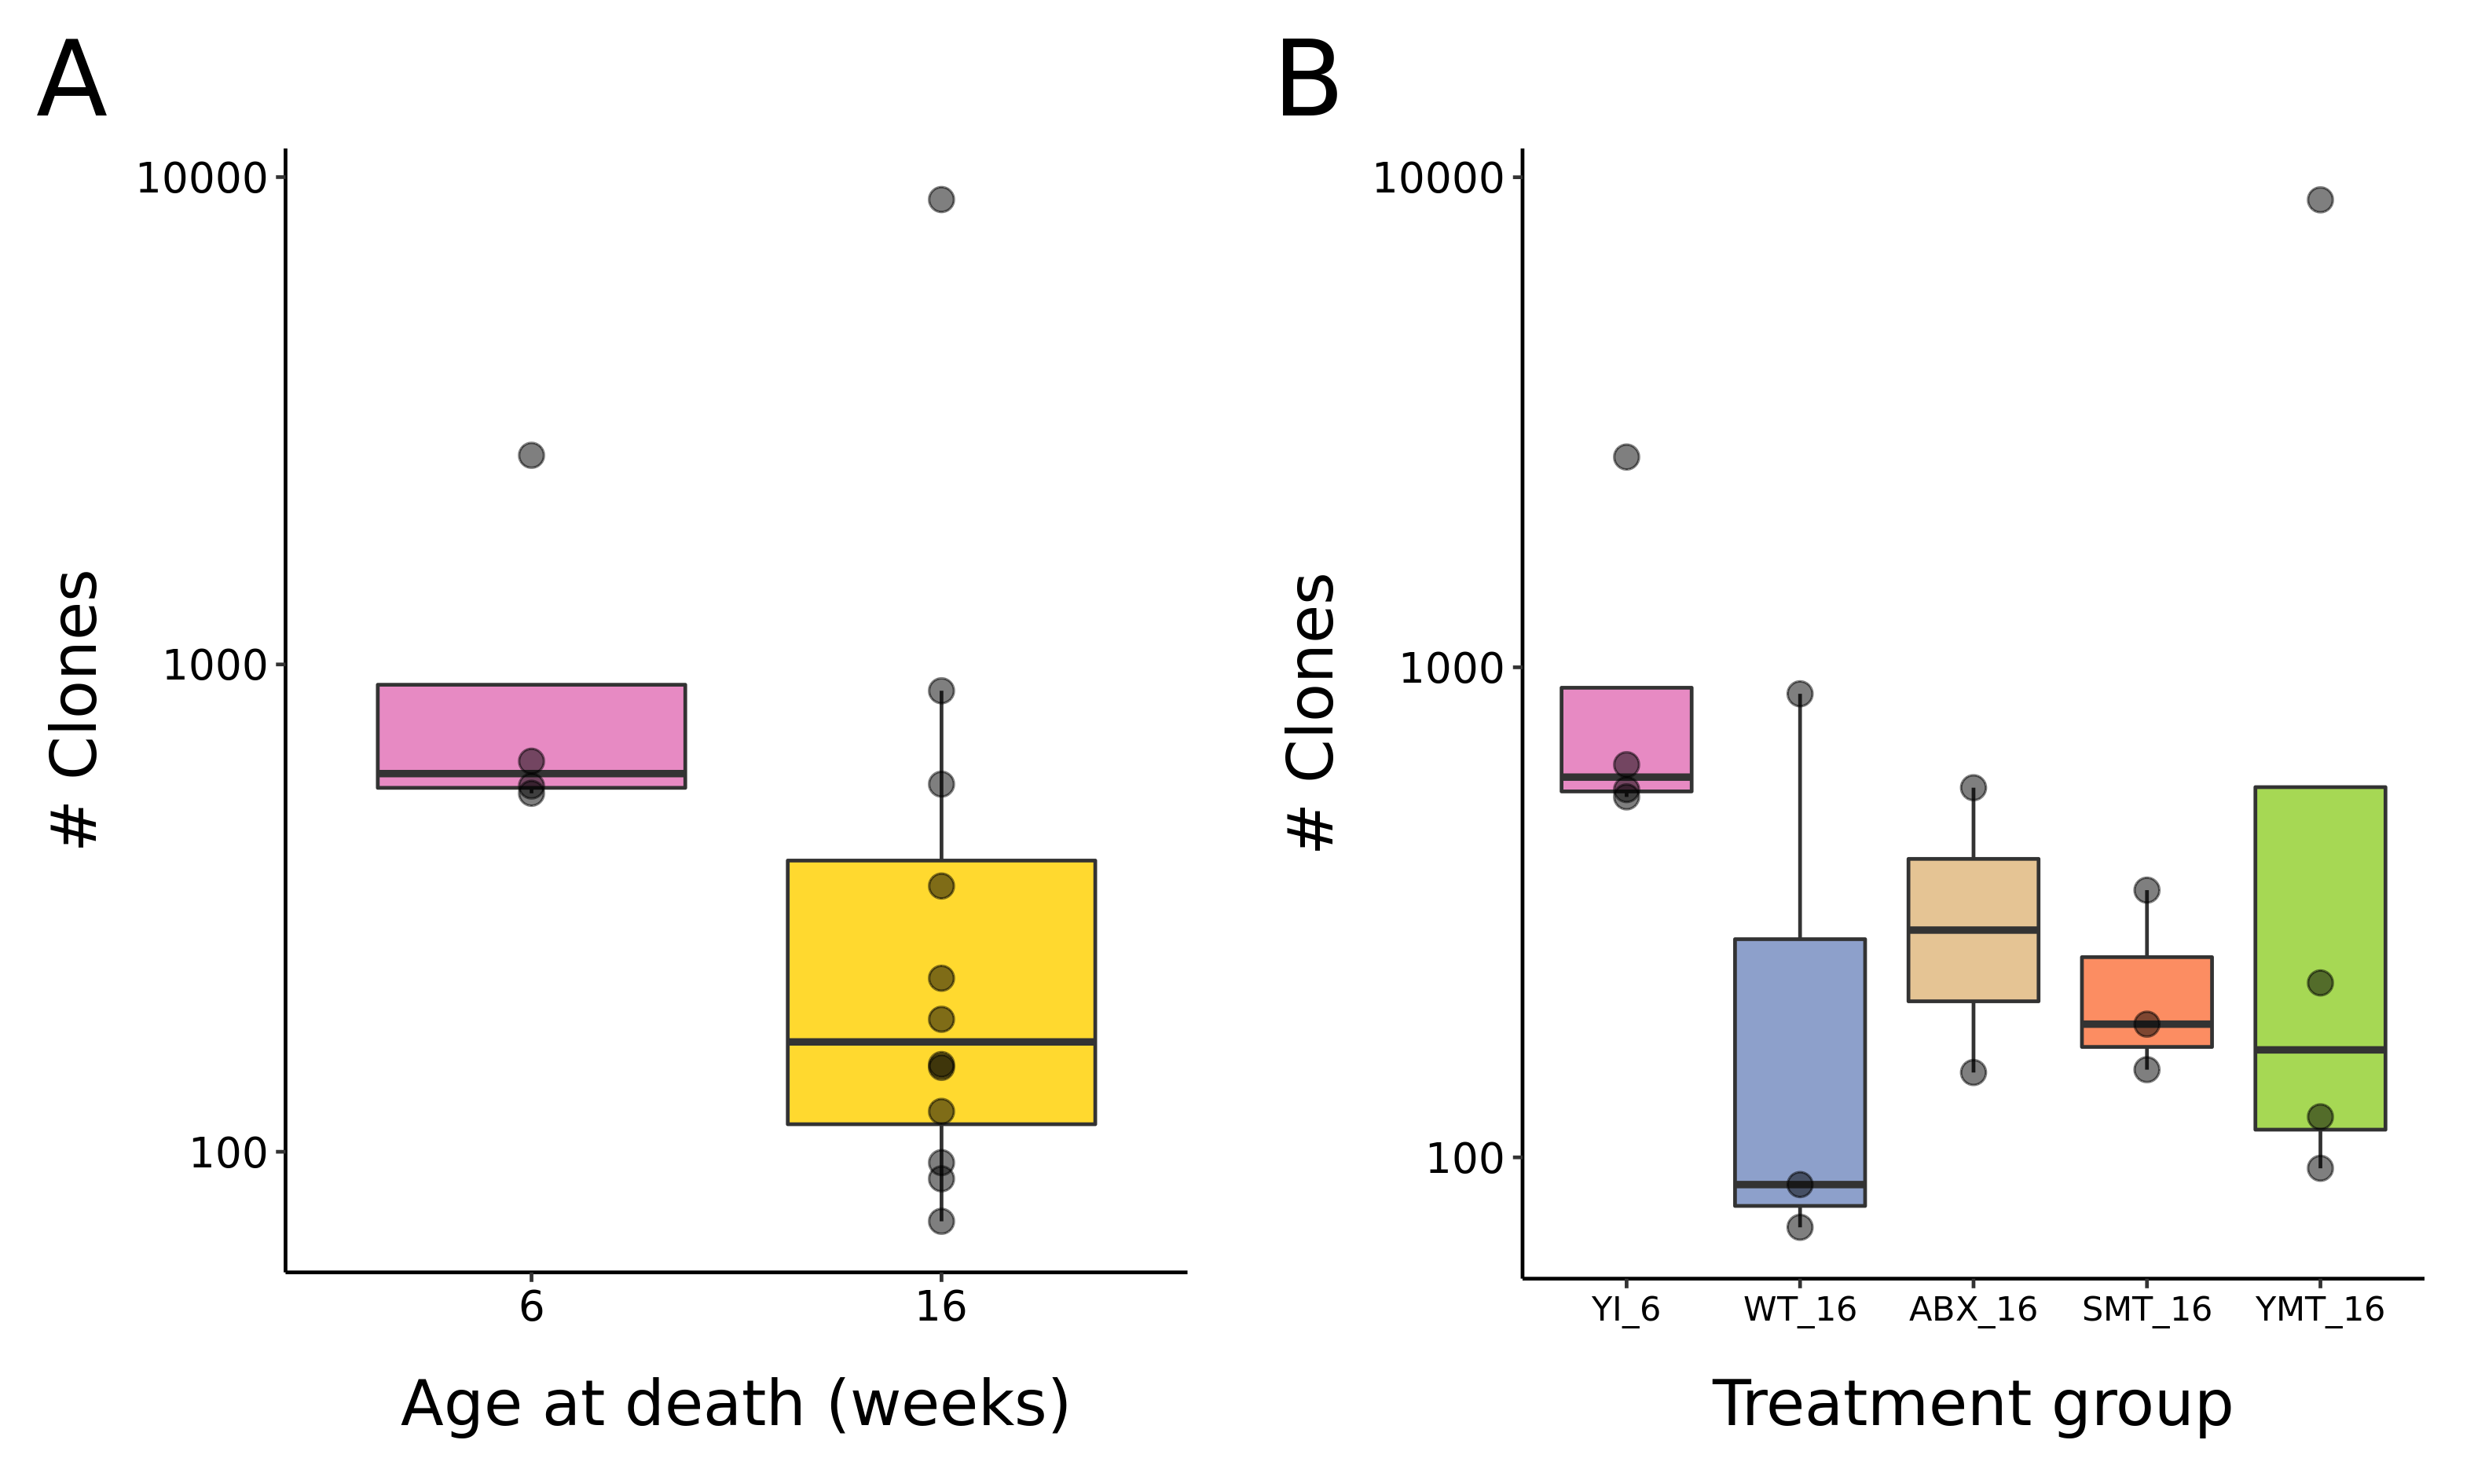
\includegraphics[width = 0.8\textwidth]{/home/will/Documents/thesis/_Figures/png/igseq-gut-nclones.png}
\caption[Number of clones in the \igseq gut dataset]{\textbf{Number of clones in the \igseq gut dataset:} Boxplots of clonal counts for each individual in the \igseq gut dataset, grouped by age at death (A) or treatment group (B). The apparent decline in clonal count with age is not significant (Kruskal-Wallis analysis of variance, $p=\embed{_Figures/txt/igseq-gut-nclones-kruskal-age-p.txt}$), and there is also no significant effect of treatment group on clonal count (Kruskal-Wallis analysis of variance, $p=\embed{_Figures/txt/igseq-gut-nclones-kruskal-group-p.txt}$).}
\label{fig:igseq-gut-nclones}
\end{figure}

\begin{figure}
\centering
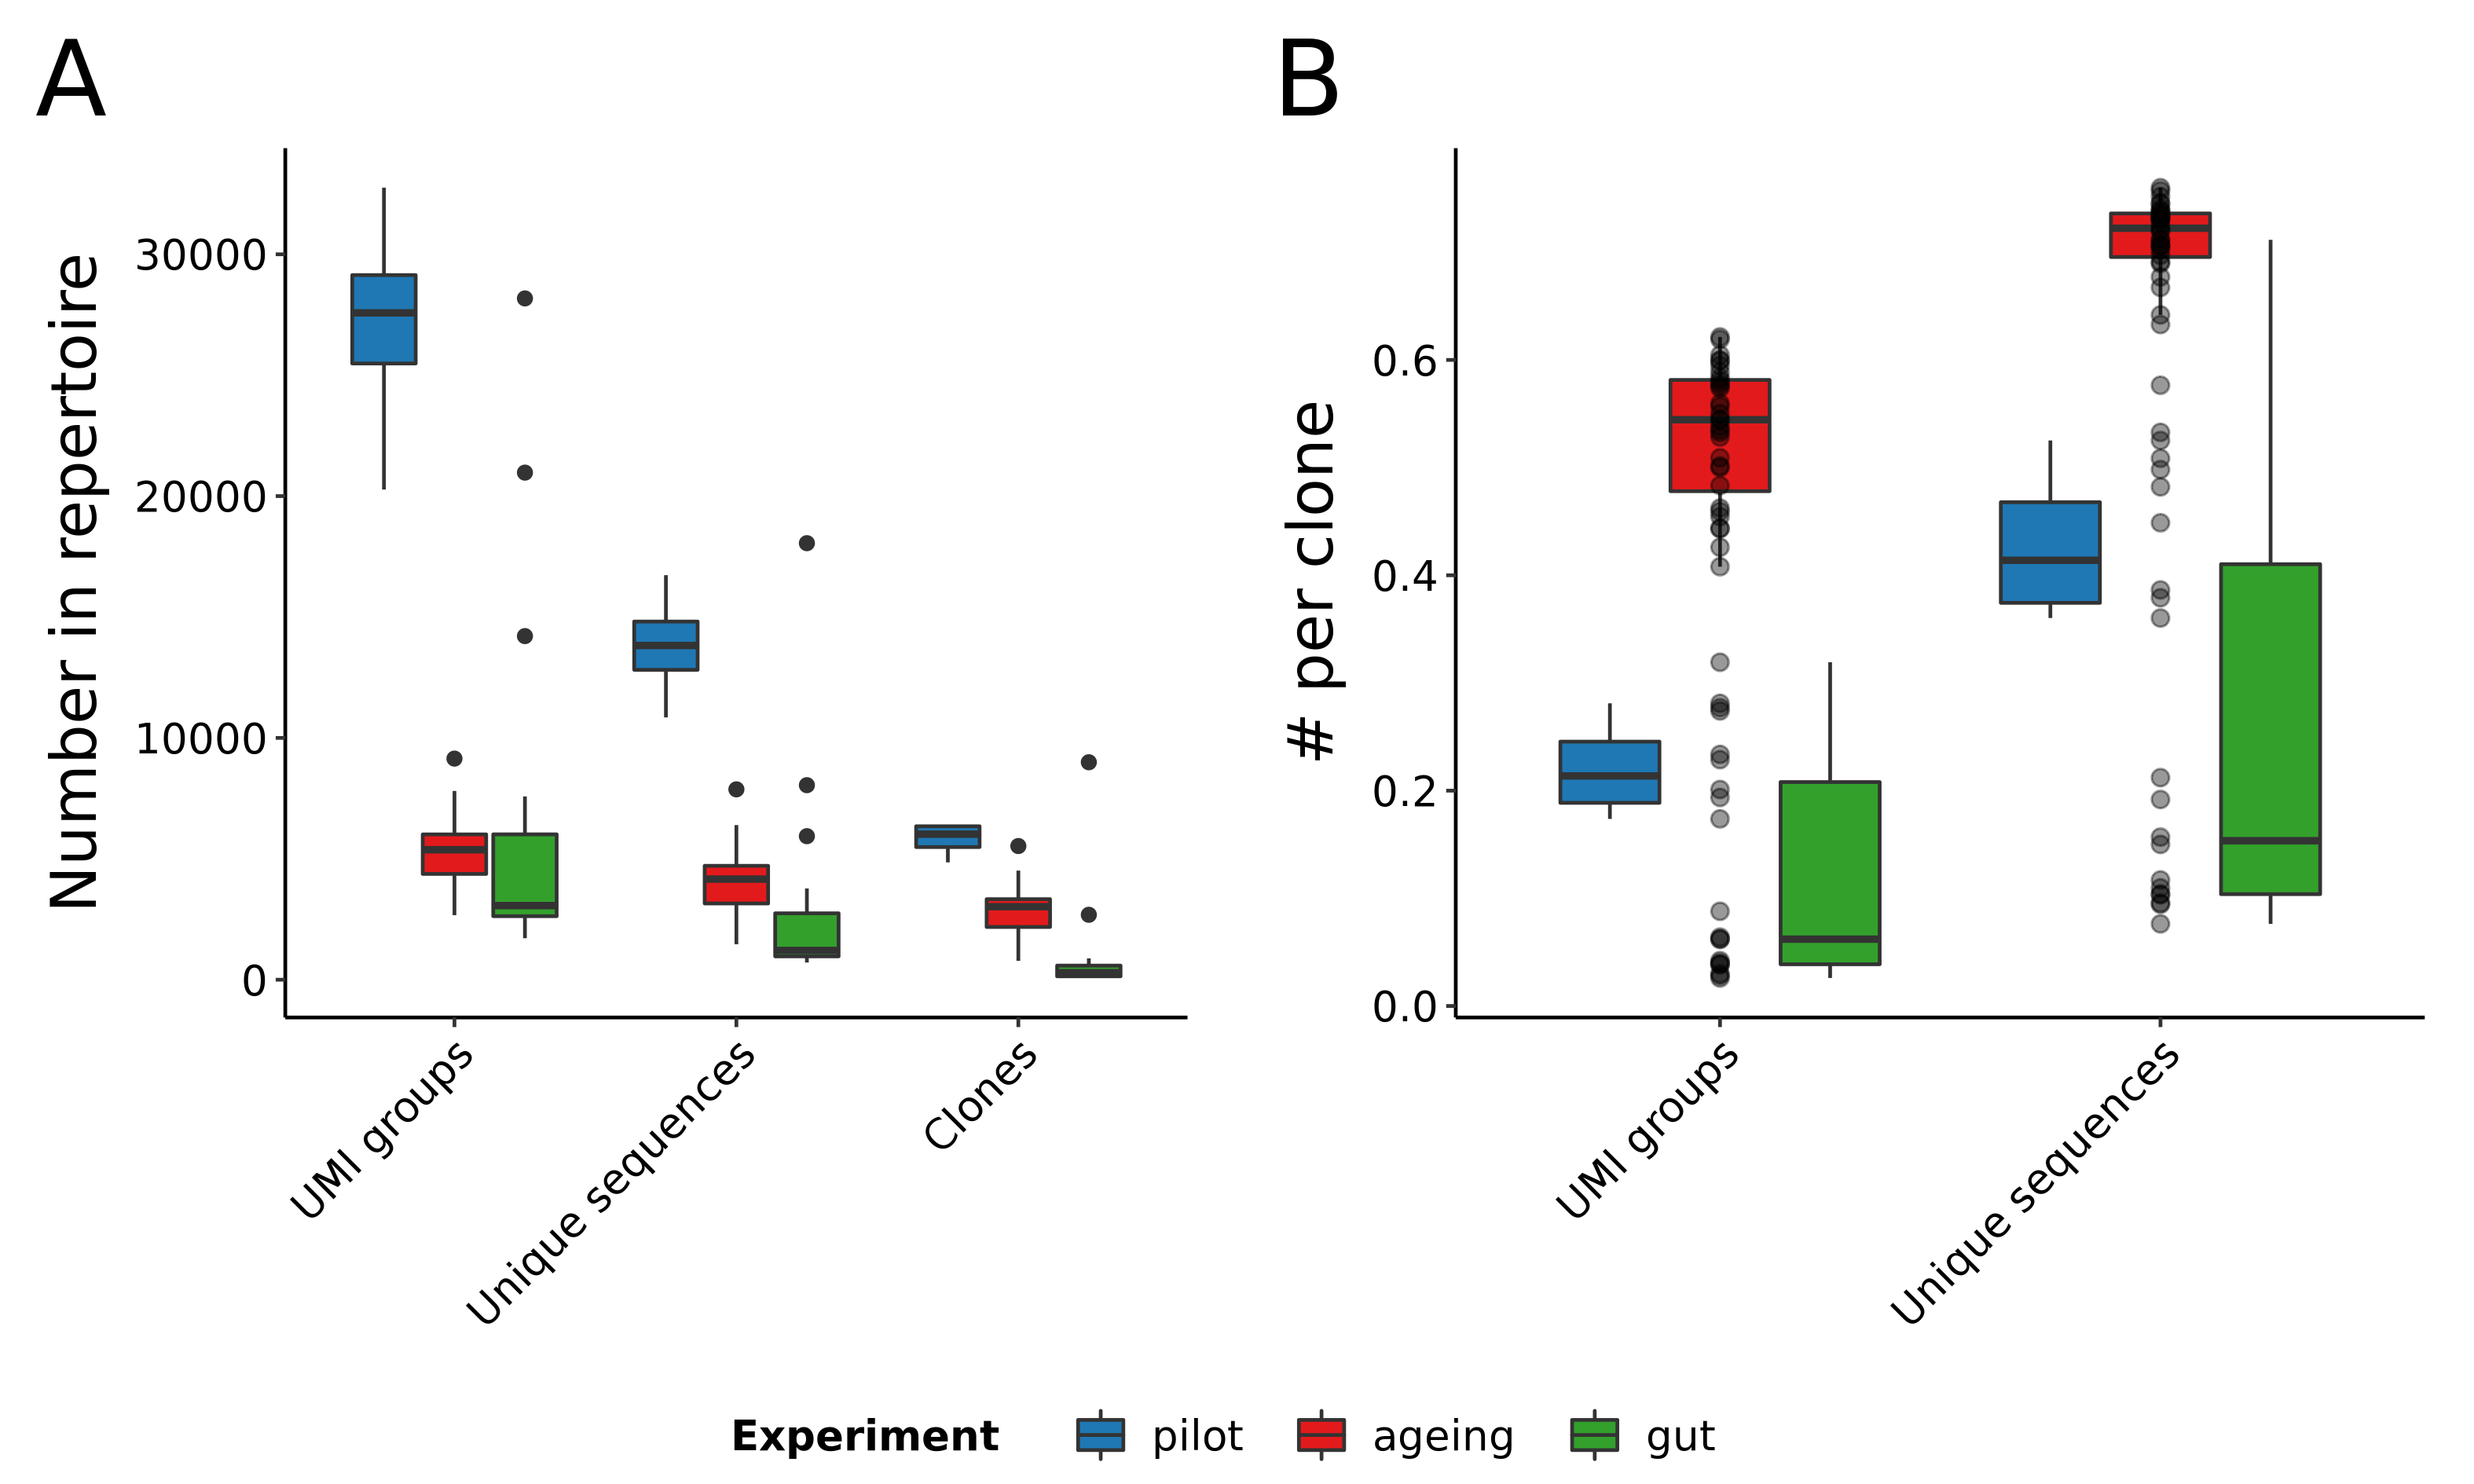
\includegraphics[width = 0.9\textwidth]{_Figures/png/igseq-comparative-metrics}
\begin{subfigure}{0em}
\phantomsubcaption{}
\label{fig:igseq-comparative-metrics-abs}
\end{subfigure}
\begin{subfigure}{0em}
\phantomsubcaption{}
\label{fig:igseq-comparative-metrics-rel}
\end{subfigure}
\caption[Comparison of clonal counts between \igseq experiments]{\textbf{Comparison of clonal counts between \igseq experiments:} Boxplots comparing different count metrics between the \igseq pilot, ageing and gut datasets, demonstrating the reduced absolute and relative clonal counts in the latter. (A) Absolute numbers of UMI groups, unique sequences and clones in each dataset. (B) Relative numbers of UMI groups and unique sequences per clone.}
\label{fig:igseq-comparative-metrics}
\end{figure}

In order to determine whether the apparent difference in clonal richness between the gut and other datasets is real, therefore, I performed rarefaction analysis, measuring the number of clones in repeated downsamplings of UMI groups from each dataset, along with the P20. The results for the rarefied clonal counts (\Cref{fig:igseq-rarefied-clone-counts}) confirm the results from \Cref{fig:igseq-comparative-metrics}: at any given downsampling size, the great majority of repertoires from the gut dataset contain far fewer clones than the repertoires in the pilot or ageing datasets. The gut repertoires also show a much greater degree of dominance by the largest clones in each repertoire (\Cref{fig:igseq-rarefied-clone-p20}), with over 85\% of gut samples exhibiting greater asymptotic P20 than over 90\% of ageing or pilot individuals and over 65\% exhibiting higher asymptotic P20 than any sample in either of the other experiments. In both cases (clonal counts and P20), a small minority of individuals deviate strongly from the general trend, exhibiting clonal counts and P20 values more consistent with those seen in the pilot and ageing experiments; however, only one individual (1412, from the 6-week-old untreated group) is an outlier in both clonal count and P20 value.

\begin{figure}
\centering
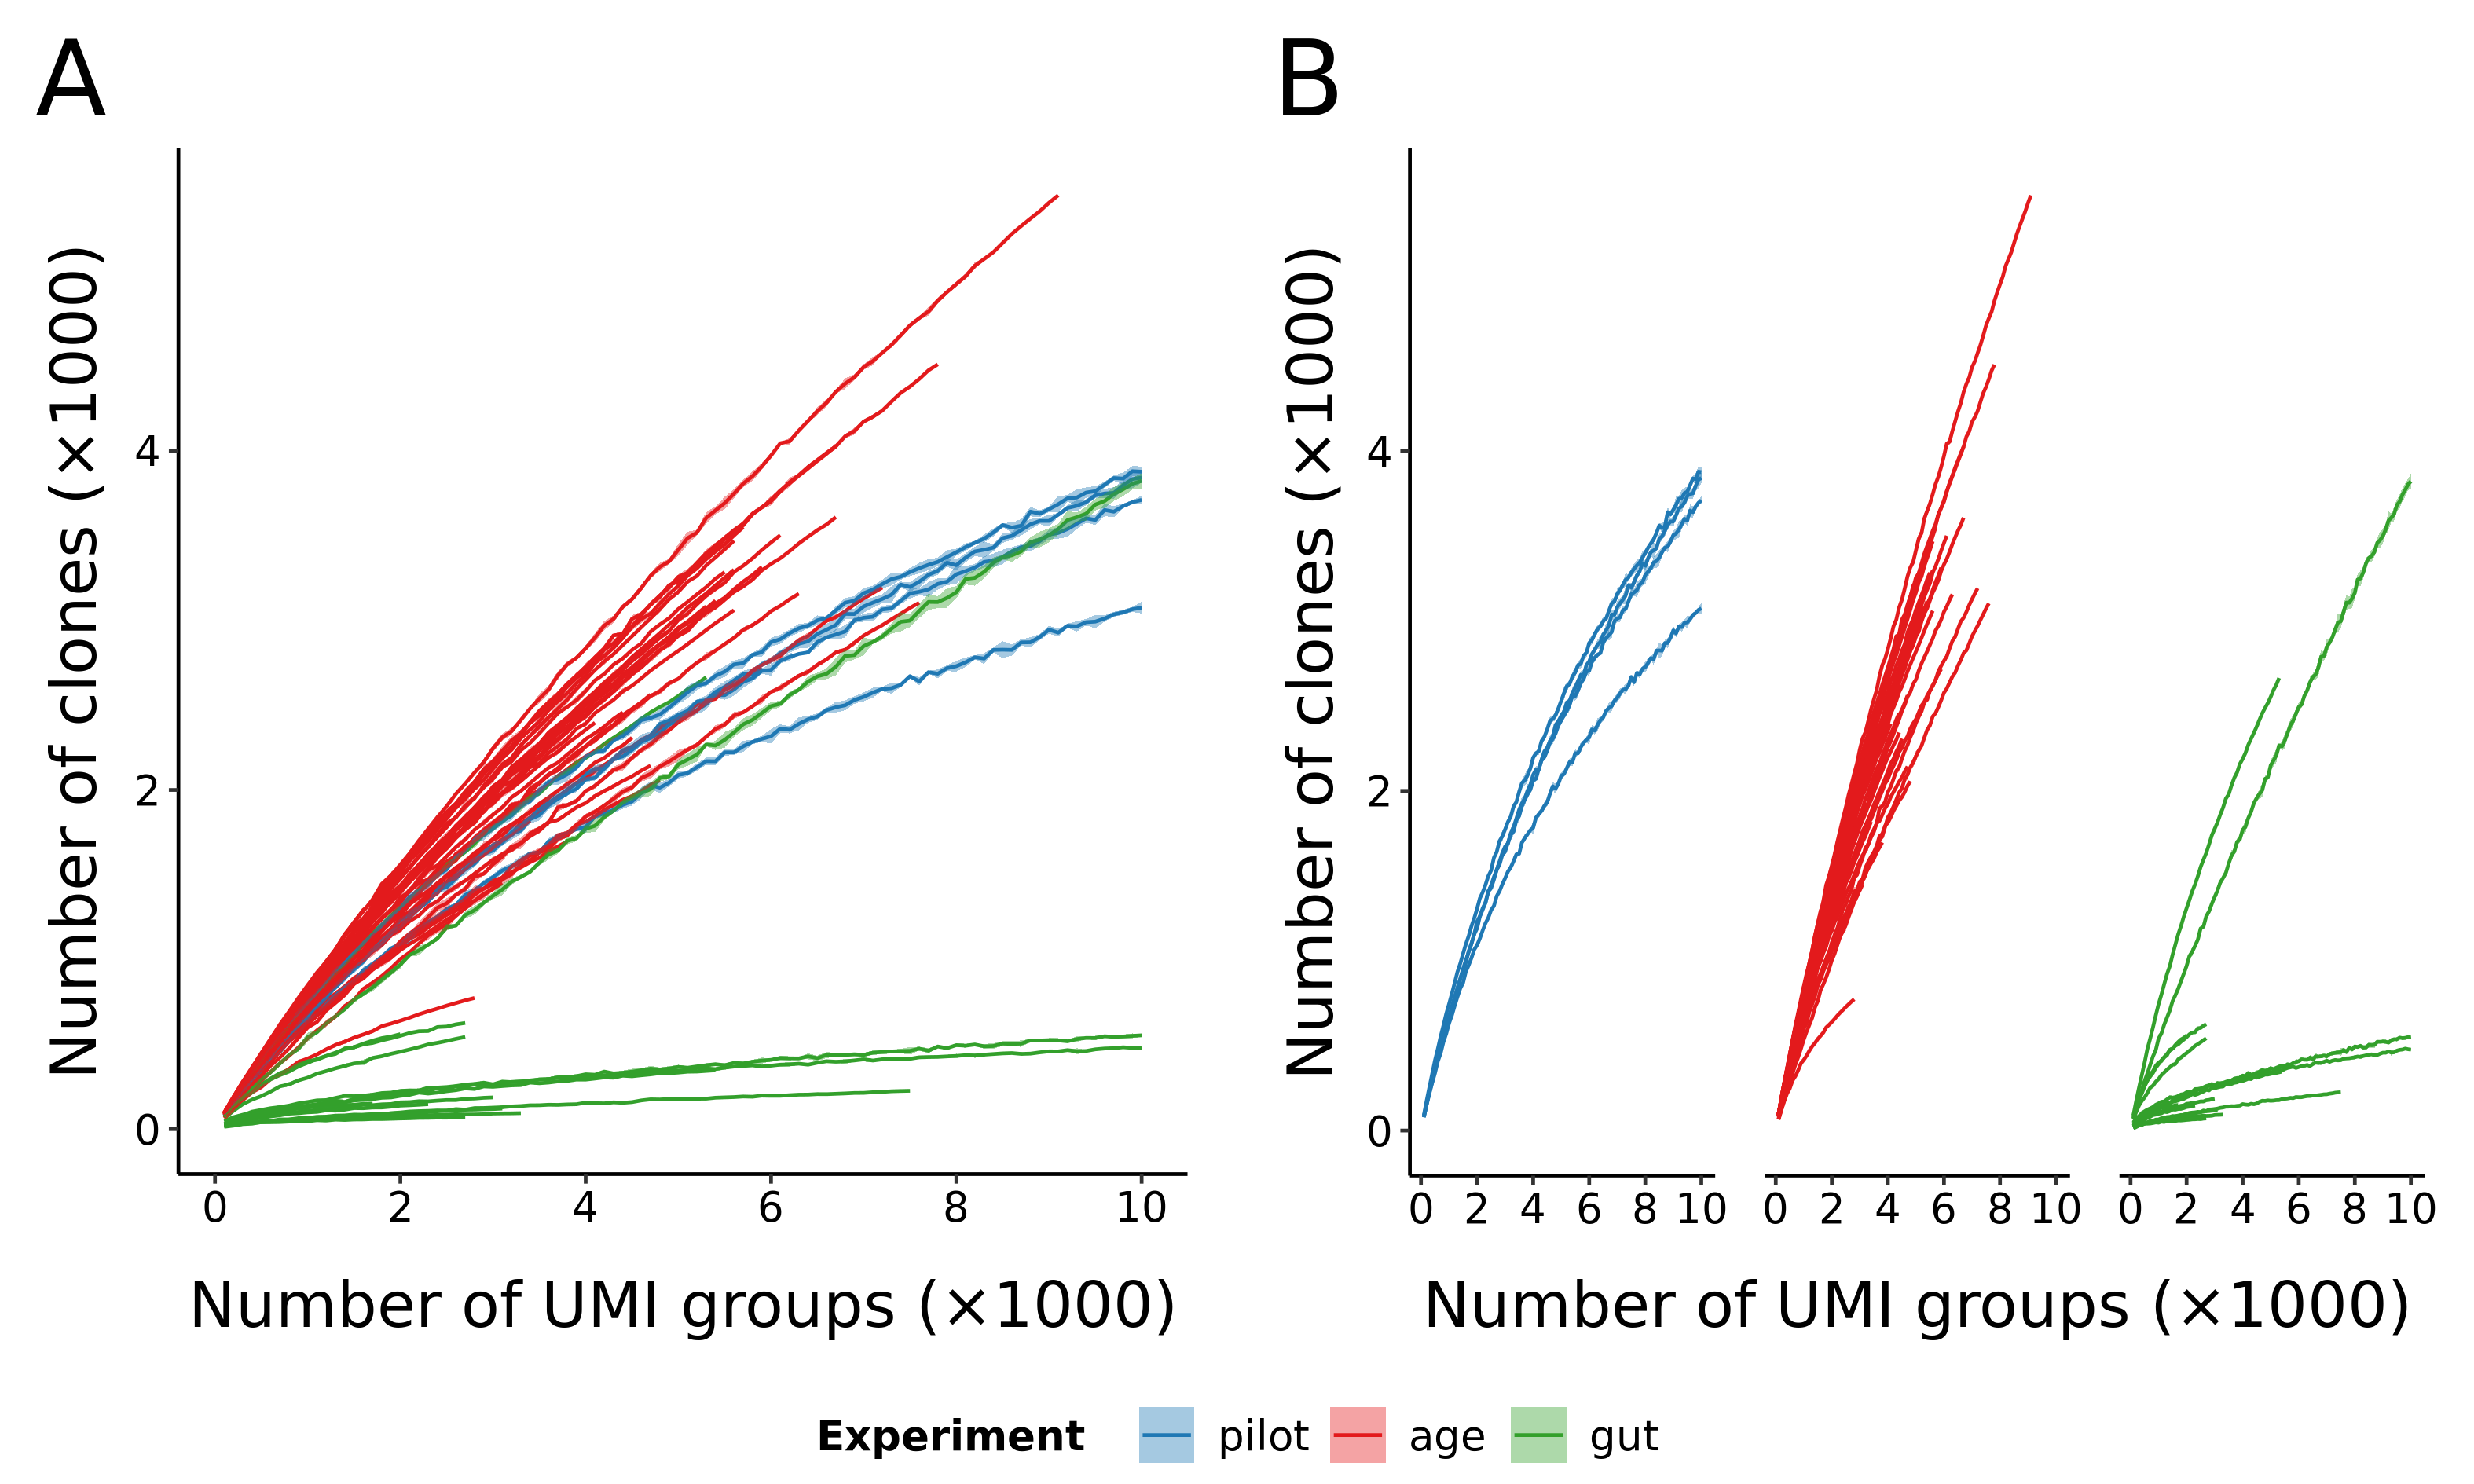
\includegraphics[width = 0.9\textwidth]{_Figures/png/igseq-rarefied-clone-counts}
\begin{subfigure}{0em}
\phantomsubcaption{}
\label{fig:igseq-rarefied-clone-counts-all}
\end{subfigure}
\begin{subfigure}{0em}
\phantomsubcaption{}
\label{fig:igseq-rarefied-clone-counts-facets}
\end{subfigure}
\caption[Comparative rarefaction analysis of clonal counts in \igseq experiments]{\textbf{Comparative rarefaction analysis of clonal counts in \igseq experiments:} Rarefaction analysis of clonal counts in turquoise killifish repertoires from the \igseq pilot, ageing and gut-microbiota-transfer experiments, displayed together (B) and separately by experiment (B). Lines and shaded regions indicate the mean and standard deviation, respectively, over twenty replicates per sample size.}
\label{fig:igseq-rarefied-clone-counts}
\end{figure}

\begin{figure}
\centering
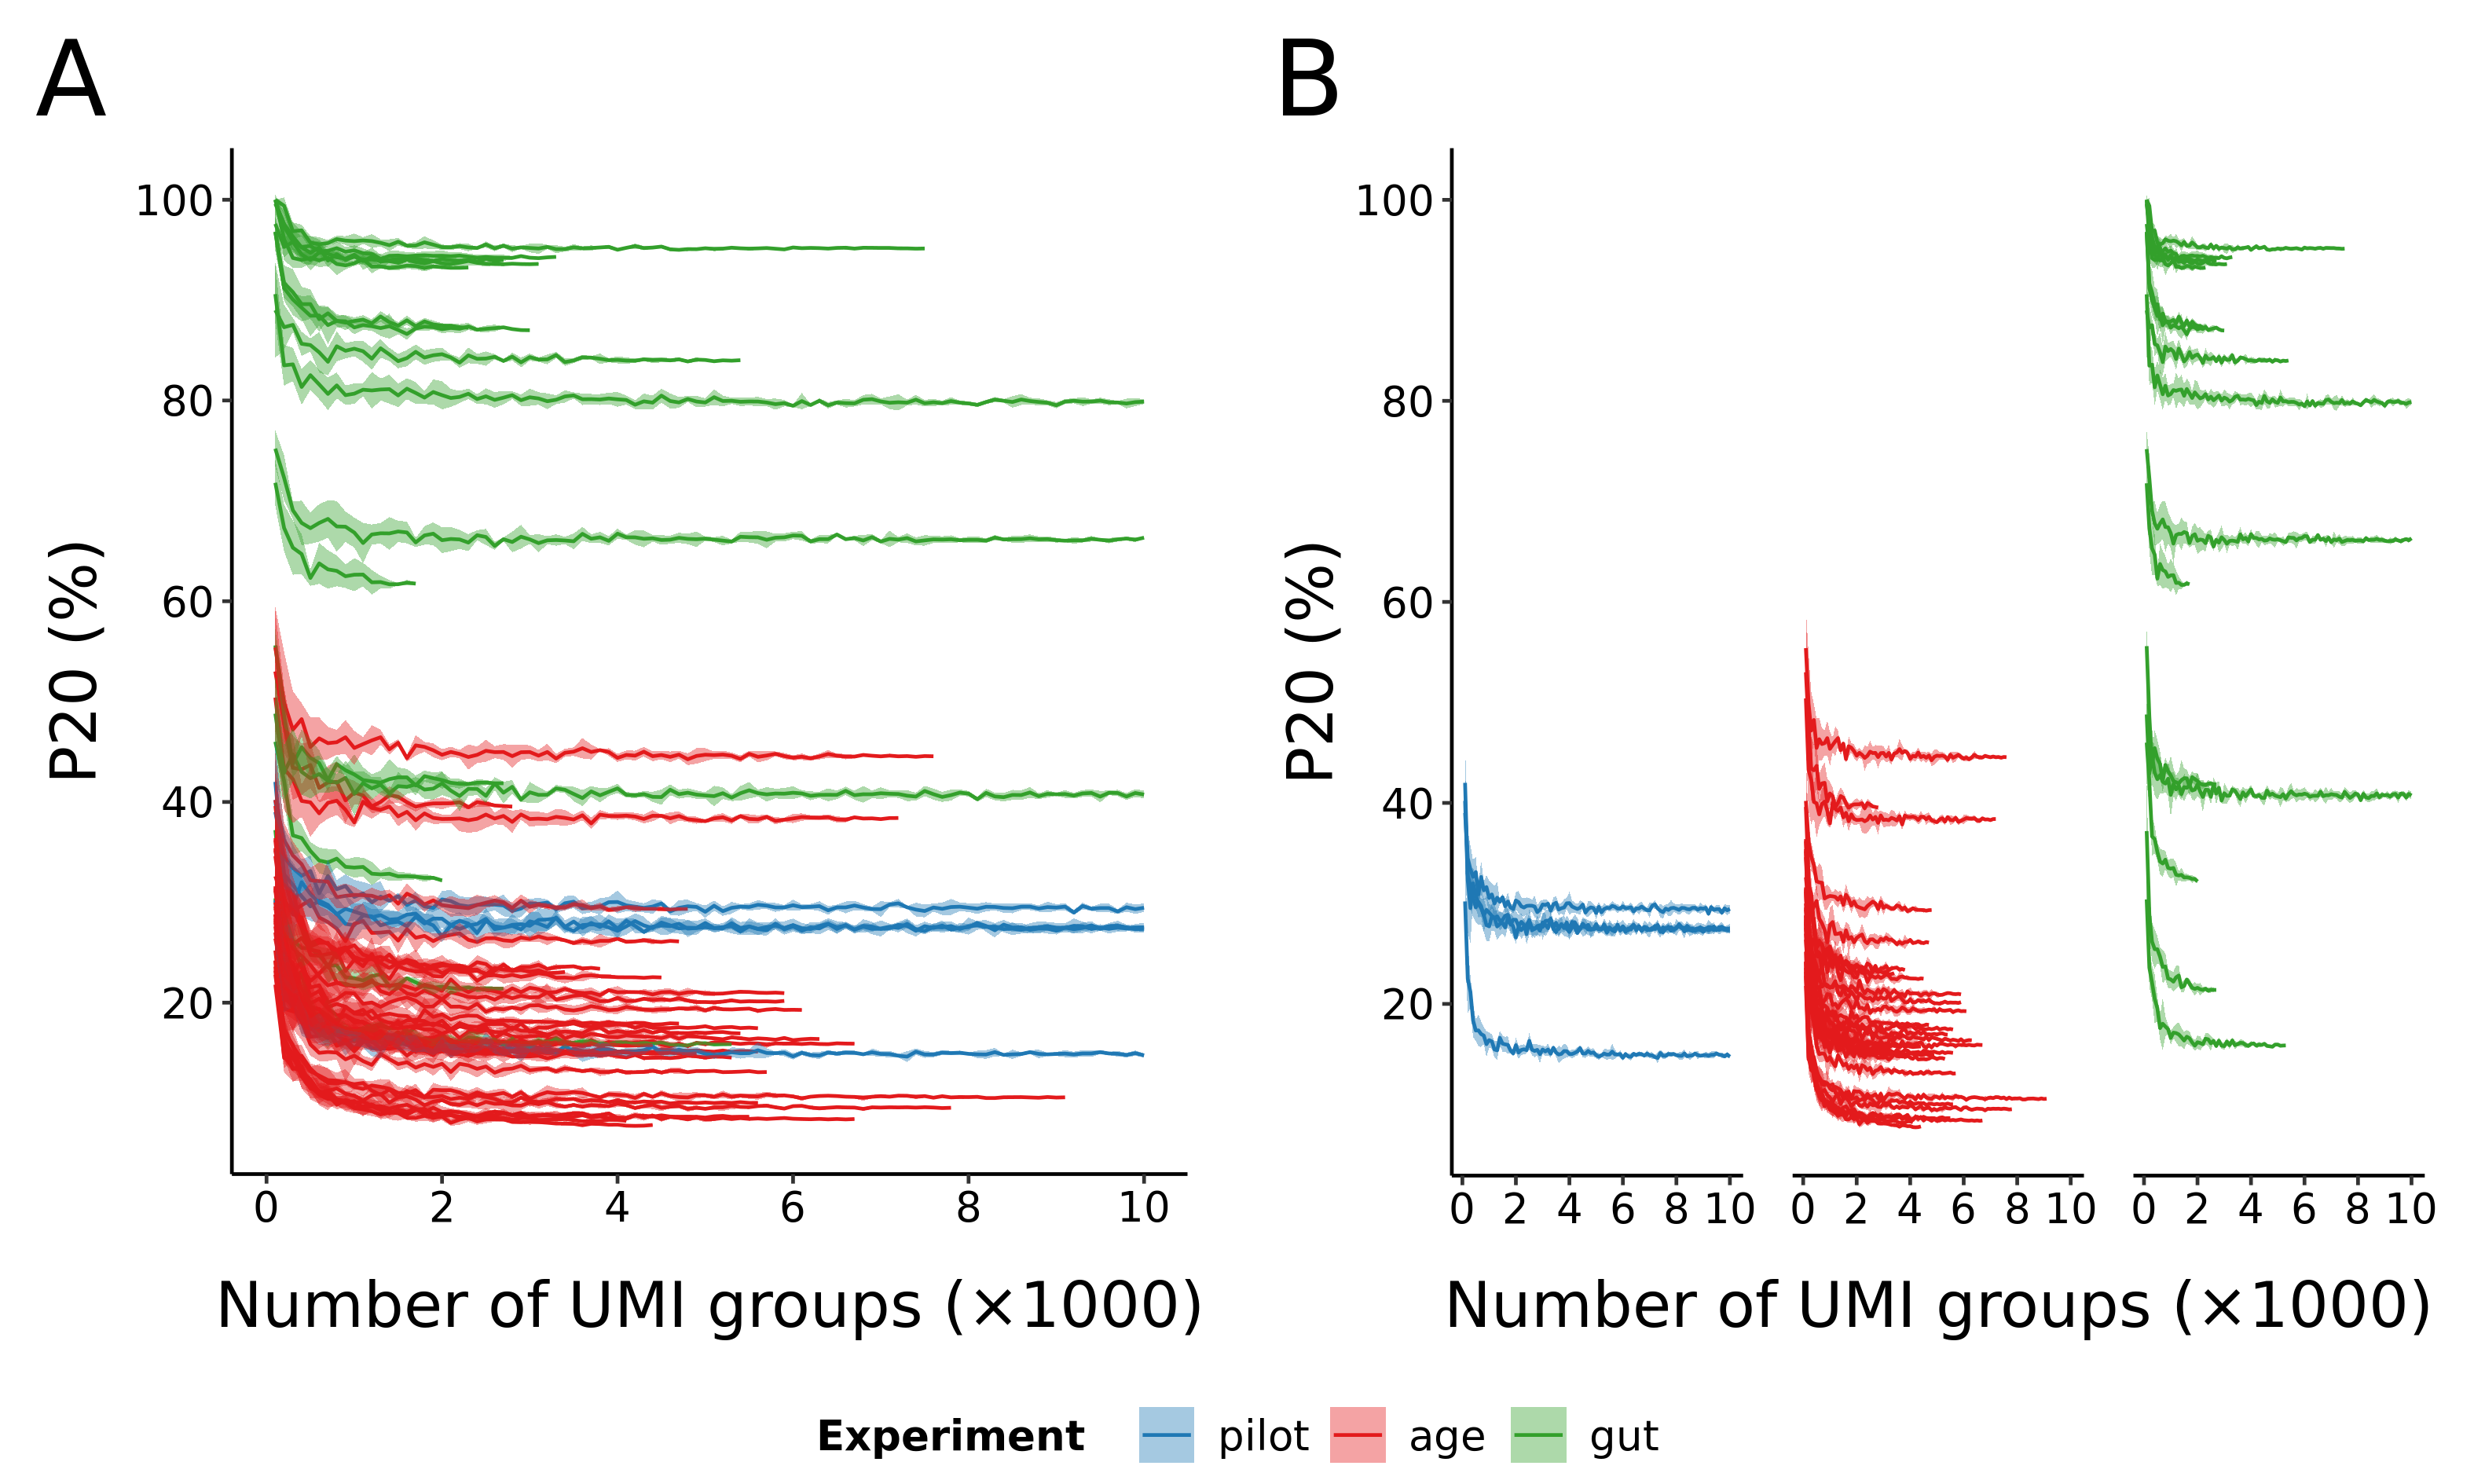
\includegraphics[width = 0.9\textwidth]{_Figures/png/igseq-rarefied-clone-p20}
\begin{subfigure}{0em}
\phantomsubcaption{}
\label{fig:igseq-rarefied-clone-p20-all}
\end{subfigure}
\begin{subfigure}{0em}
\phantomsubcaption{}
\label{fig:igseq-rarefied-clone-p20-facets}
\end{subfigure}
\caption[Comparative rarefaction analysis of P20 scores in \igseq experiments]{\textbf{Comparative rarefaction analysis of P20 scores in \igseq experiments:} Rarefaction analysis of the proportion of each turquoise killifish repertoire occupied by the twenty largest clones (P20) in the \igseq pilot, ageing and gut-microbiota-transfer experiments, displayed together (A) and separately by experiment (B). Lines and shaded regions indicate the mean and standard deviation, respectively, over twenty replicates per sample size.}
\label{fig:igseq-rarefied-clone-p20}
\end{figure}

The combination of low clonal counts and elevated P20 indicated by \Cref{fig:igseq-rarefied-clone-counts,fig:igseq-rarefied-clone-p20} suggests that the killifish gut repertoire contains many fewer small, \naive clones than the whole-body repertoire, and is consequently much more strongly dominated by a comparatively small number of expanded clones. This hypothesis is confirmed when the rarefied clonal counts are separated by clone size (\Cref{fig:igseq-rarefied-clone-counts-size}): while the number of small clones (containing fewer than 5 unique sequences) in the gut repertoires is again much smaller than in the other experiments (\Cref{fig:igseq-rarefied-clone-counts-small}), the number of large clones (containing at least 5 unique sequences) is roughly the same (\Cref{fig:igseq-rarefied-clone-counts-large}), and as a consequence the proportion of large clones is much higher in most gut repertoires than in the whole body (\Cref{fig:igseq-rarefied-clone-counts-large-pc}). This difference between the gut and whole-body repertoires makes sense: unlike the gut repertoire, the whole body repertoire includes clones from primary lymphoid organs (in particular, the anterior kidney), and so could be expected to contain a much larger number of small, \naive clones. Furthermore, as a site of extensive interaction between the host and the gut microbiota, the gut provides many opportunities for its resident B-cells to encounter foreign antigens\parencite{caruso2009immunosenescence} , and the consequent high rate of clonal expansion is likely to further increase the extent to which the gut repertoire is dominated by large clones.

\begin{figure}
\centering
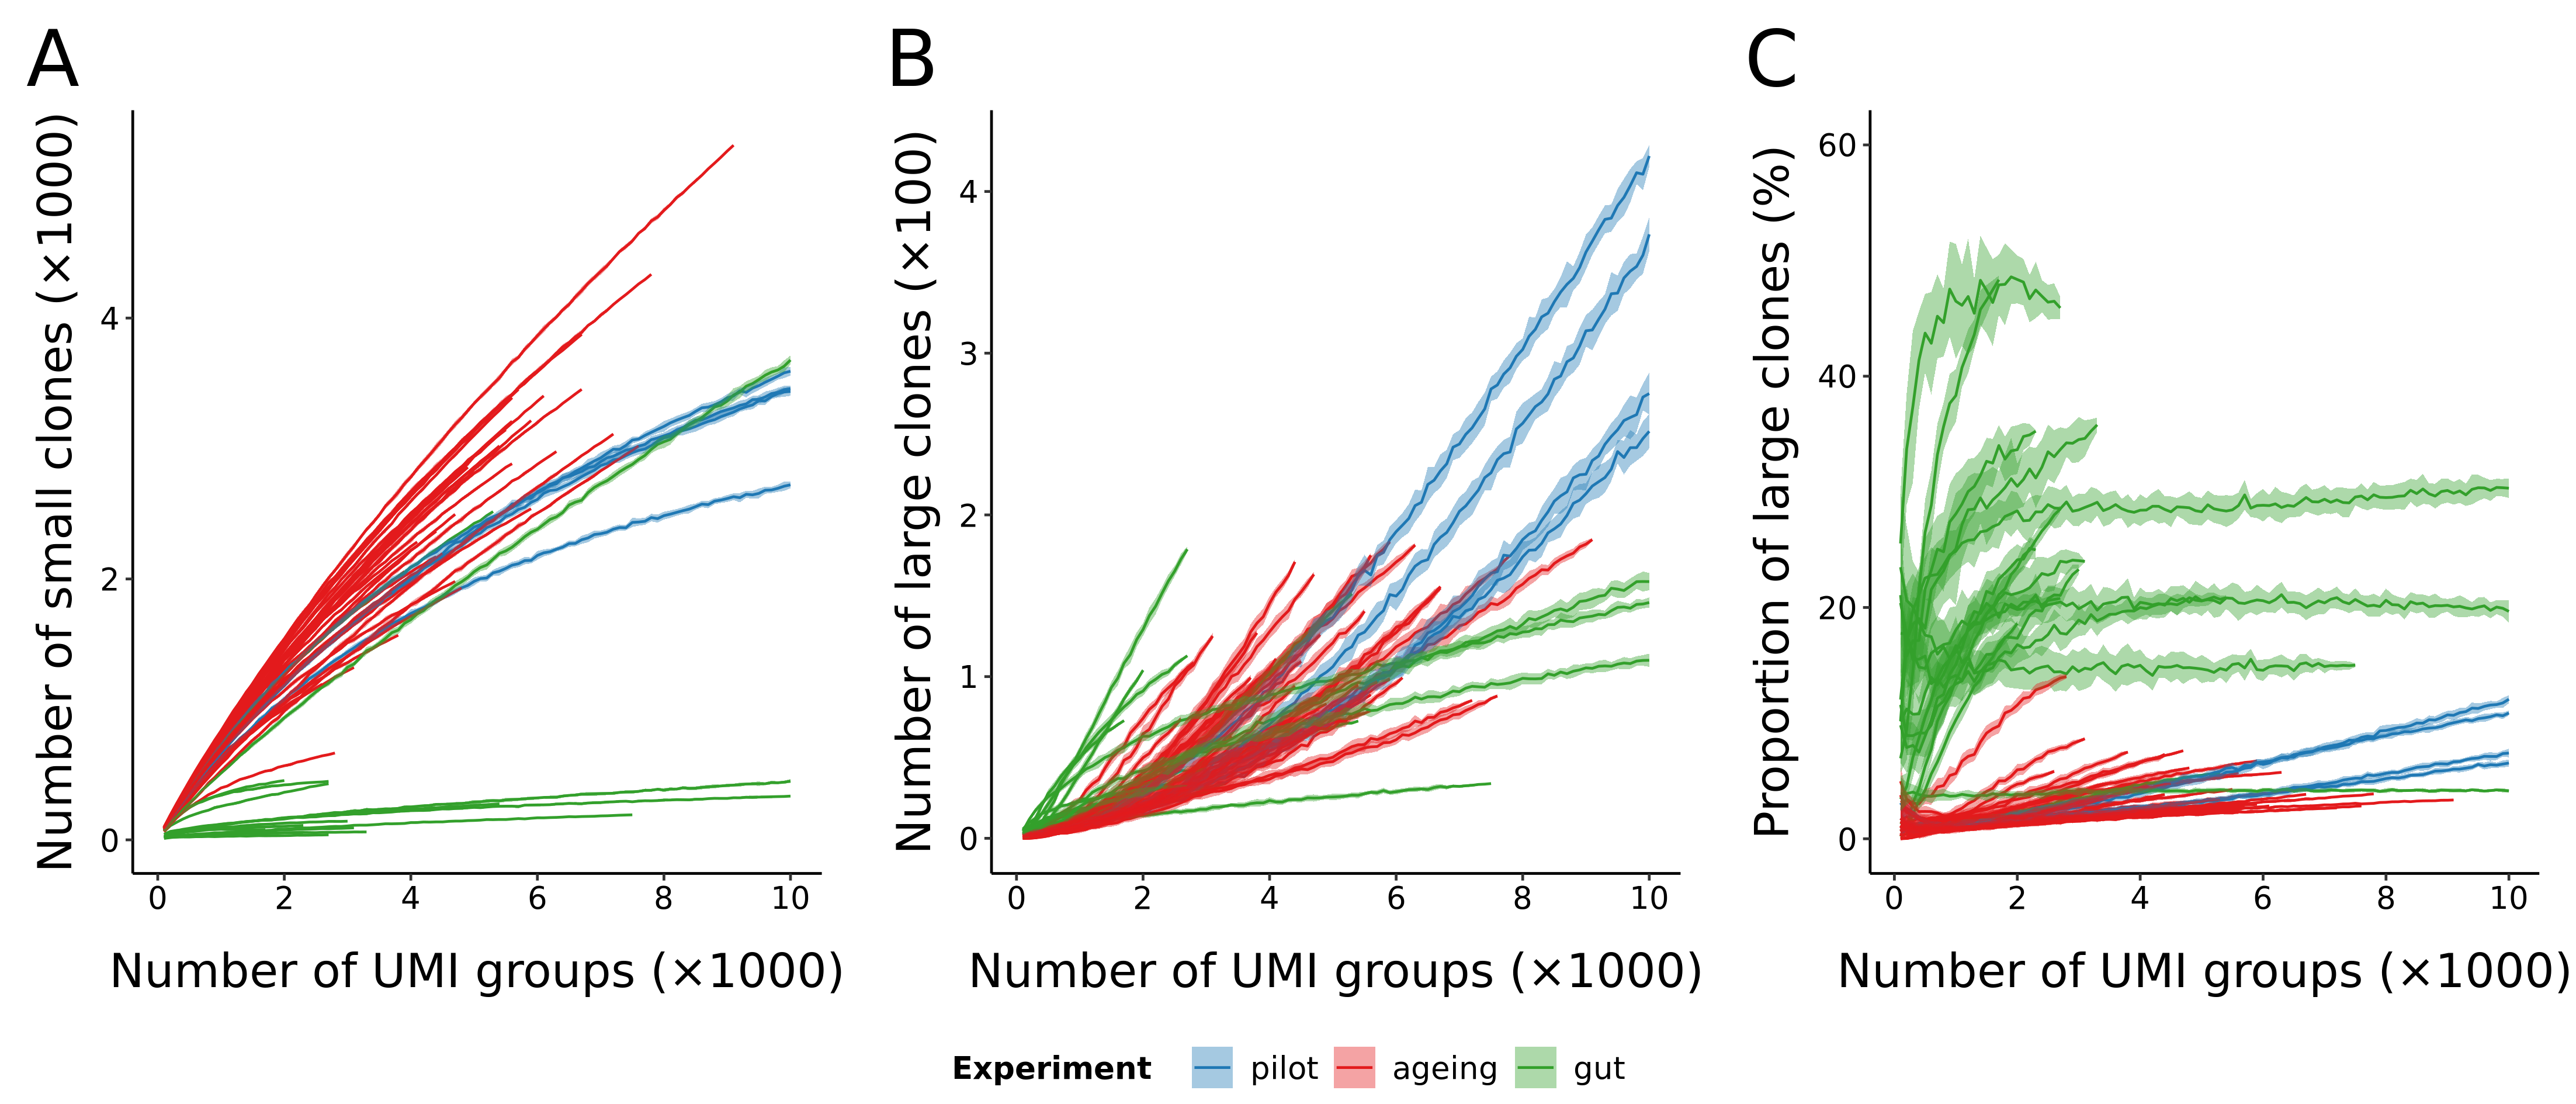
\includegraphics[width = \textwidth]{_Figures/png/igseq-rarefied-clone-counts-size}
\begin{subfigure}{0em}
\phantomsubcaption{}
\label{fig:igseq-rarefied-clone-counts-small}
\end{subfigure}
\begin{subfigure}{0em}
\phantomsubcaption{}
\label{fig:igseq-rarefied-clone-counts-large}
\end{subfigure}
\begin{subfigure}{0em}
\phantomsubcaption{}
\label{fig:igseq-rarefied-clone-counts-large-pc}
\end{subfigure}
\caption[Comparative rarefaction analysis of clonal size composition in \igseq experiments]{\textbf{Comparative rarefaction analysis of clonal size composition in \igseq experiments:} Rarefaction curves of (A) the number of small clones ($>5$ unique sequences), (B) the number of large clones ($\geq 5$ unique sequences) and (C) the proportion of clones which are large in each individual, coloured by source experiment. Lines and shaded regions indicate the mean and standard deviation, respectively, over twenty replicates per sample size.}
\label{fig:igseq-rarefied-clone-counts-size}
\end{figure}

The clonal alpha-diversity spectra for the gut dataset are shown in \Cref{fig:igseq-gut-clone-diversity-alpha}. At all diversity orders, there is a clear and drastic difference between the young (6-week-old) and old (16-week-old) groups, while the different 16-week-old treatment groups do not appear to show a strong difference in diversity. These observations are confirmed by statistical comparison of the distributions of individual diversity measurements at different diversity orders, which indicate highly significant differences in clonal repertoire diversity between young and old guts across the diversity spectrum (\Cref{fig:igseq-gut-clone-diversity-solo-age}), but no difference between treatment groups (\Cref{fig:igseq-gut-clone-diversity-solo-groups}). A similar pattern is observed for V/J-usage diversity (\Cref{fig:igseq-gut-VJ-diversity-alpha}), with a large and significant difference between young and old cohorts at many different diversity orders (\Cref{fig:igseq-gut-VJ-diversity-solo-age}) but no significant differences between 16-week-old treatment groups (\Cref{fig:igseq-gut-VJ-diversity-solo-groups}).

\begin{figure}
\centering
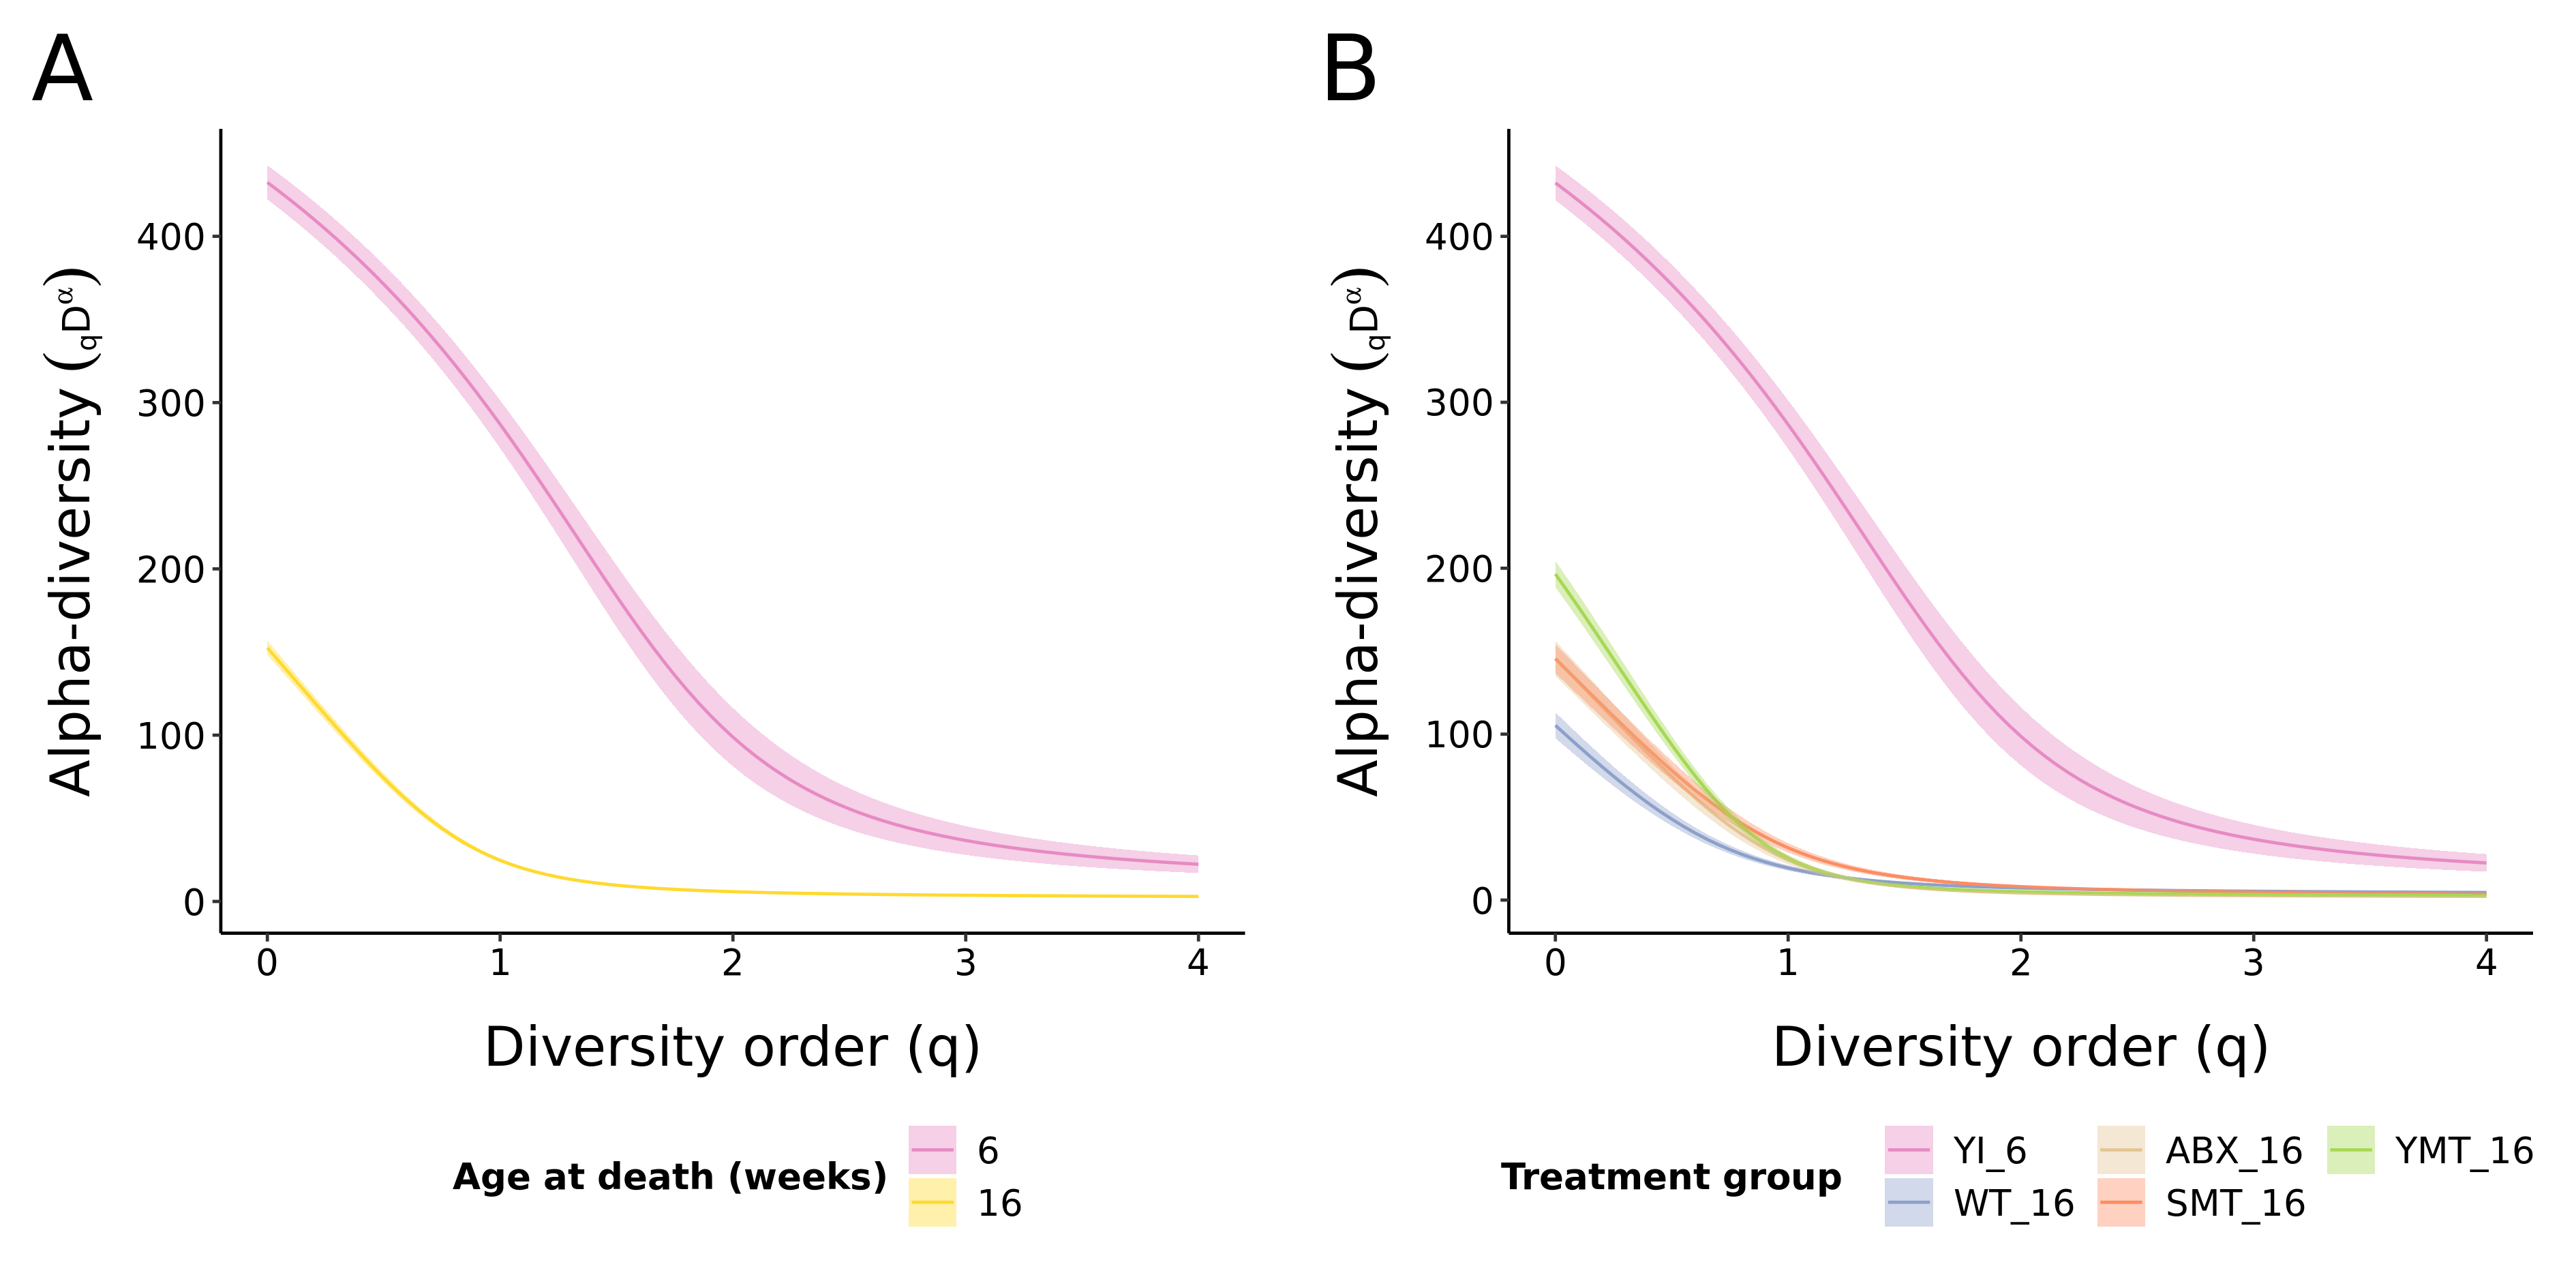
\includegraphics[width = 0.9\textwidth]{_Figures/png/igseq-gut-clone-diversity-alpha}
\begin{subfigure}{0em}
\phantomsubcaption{}
\label{fig:igseq-gut-clone-diversity-alpha-age}
\end{subfigure}
\begin{subfigure}{0em}
\phantomsubcaption{}
\label{fig:igseq-gut-clone-diversity-alpha-groups}
\end{subfigure}
\caption[Clonal alpha-diversity spectra for \igseq gut dataset]{\textbf{Clonal alpha-diversity spectra for \igseq gut dataset:} Bootstrapped alpha-diversity spectra of clone sizes for each (A) age group and (B) treatment group in the \igseq ageing dataset, as measured by number of unique sequences per clone. Shaded regions in both subfigures represent 95\,\% confidence intervals, estimated using bootstrapping.}
\label{fig:igseq-gut-clone-diversity-alpha}
\end{figure}

% TODO: Per-individual diversity spectra for supplementary

\begin{figure}
\centering
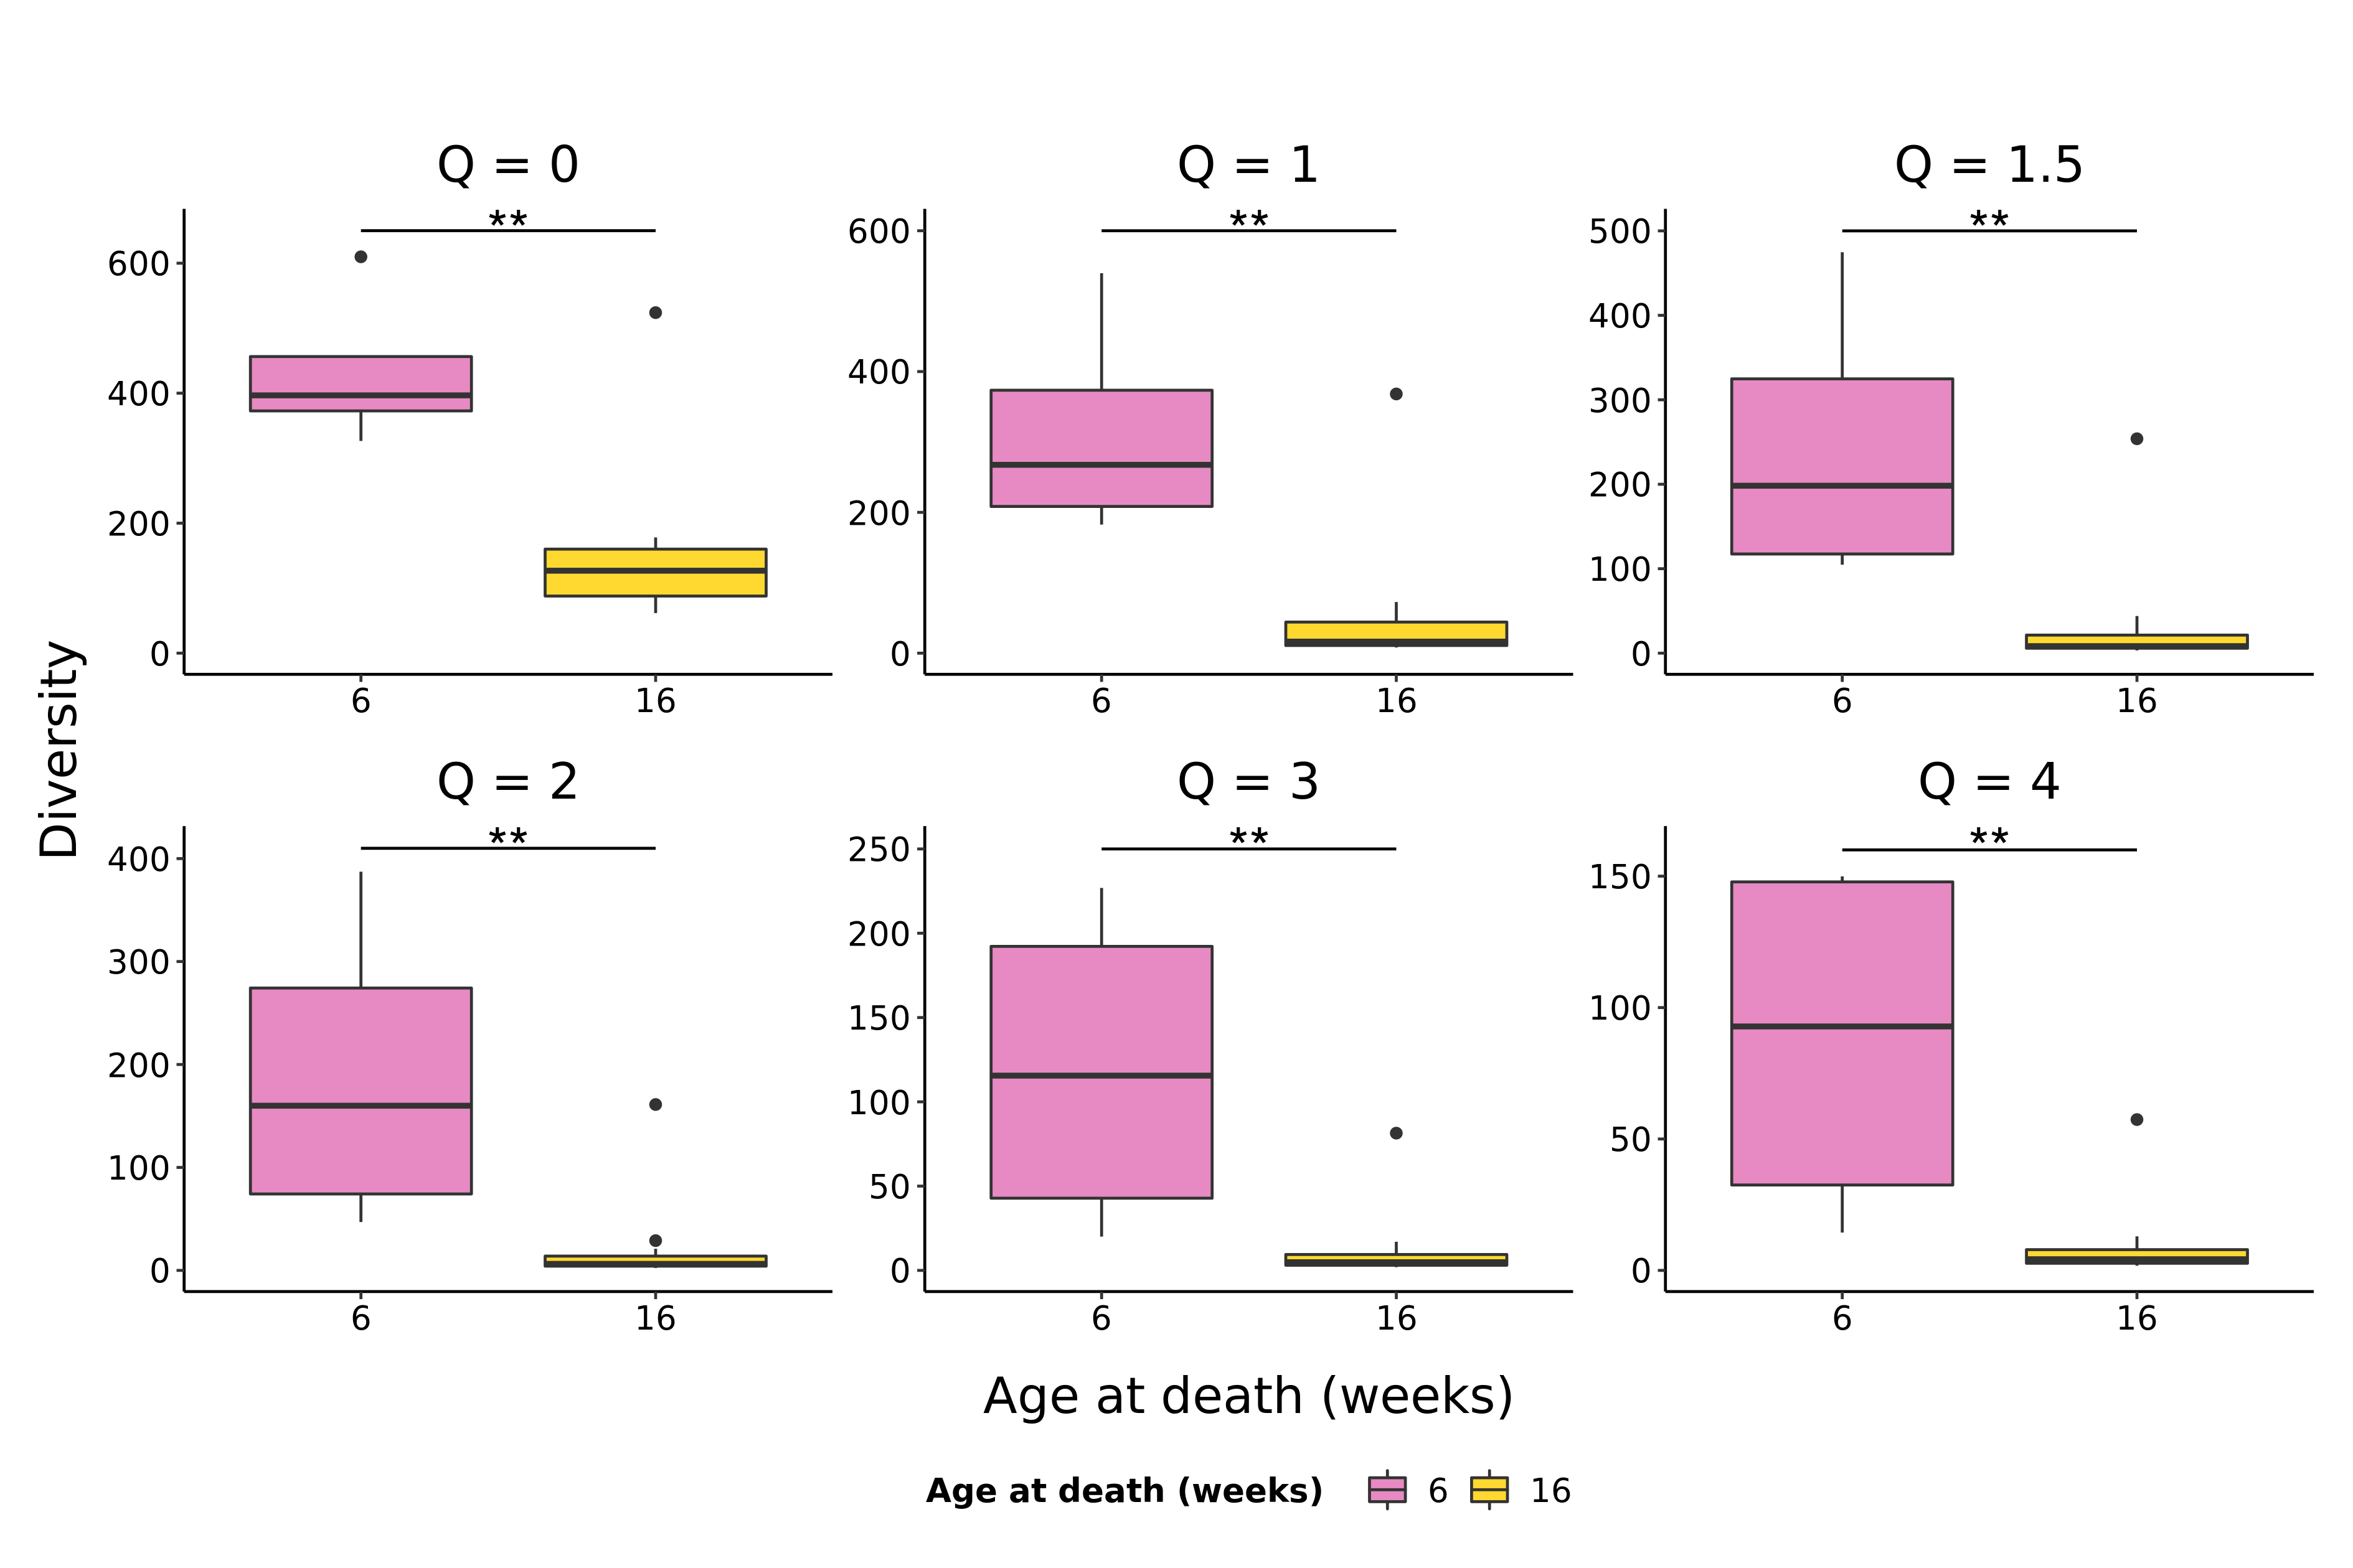
\includegraphics[width = 0.9\textwidth]{_Figures/png/igseq-gut-clone-diversity-solo-age}
\caption[Comparing clonal alpha-diversities between age groups in the \igseq gut dataset]{\textbf{Comparing clonal alpha-diversities between age groups in the \igseq gut dataset:} Boxplots of clonal Hill diversity values for the antibody repertoires of individuals of each age group in the \igseq gut dataset at a sample of diversity orders. Pairwise $p$-values are computed using nonparametric Mann–Whitney U tests ($*: 0.01 < p \leq 0.05;~**: 0.001 < p \leq 0.01;~***: p \leq 0.001$).}
\label{fig:igseq-gut-clone-diversity-solo-age}
\end{figure}

\begin{figure}
\centering
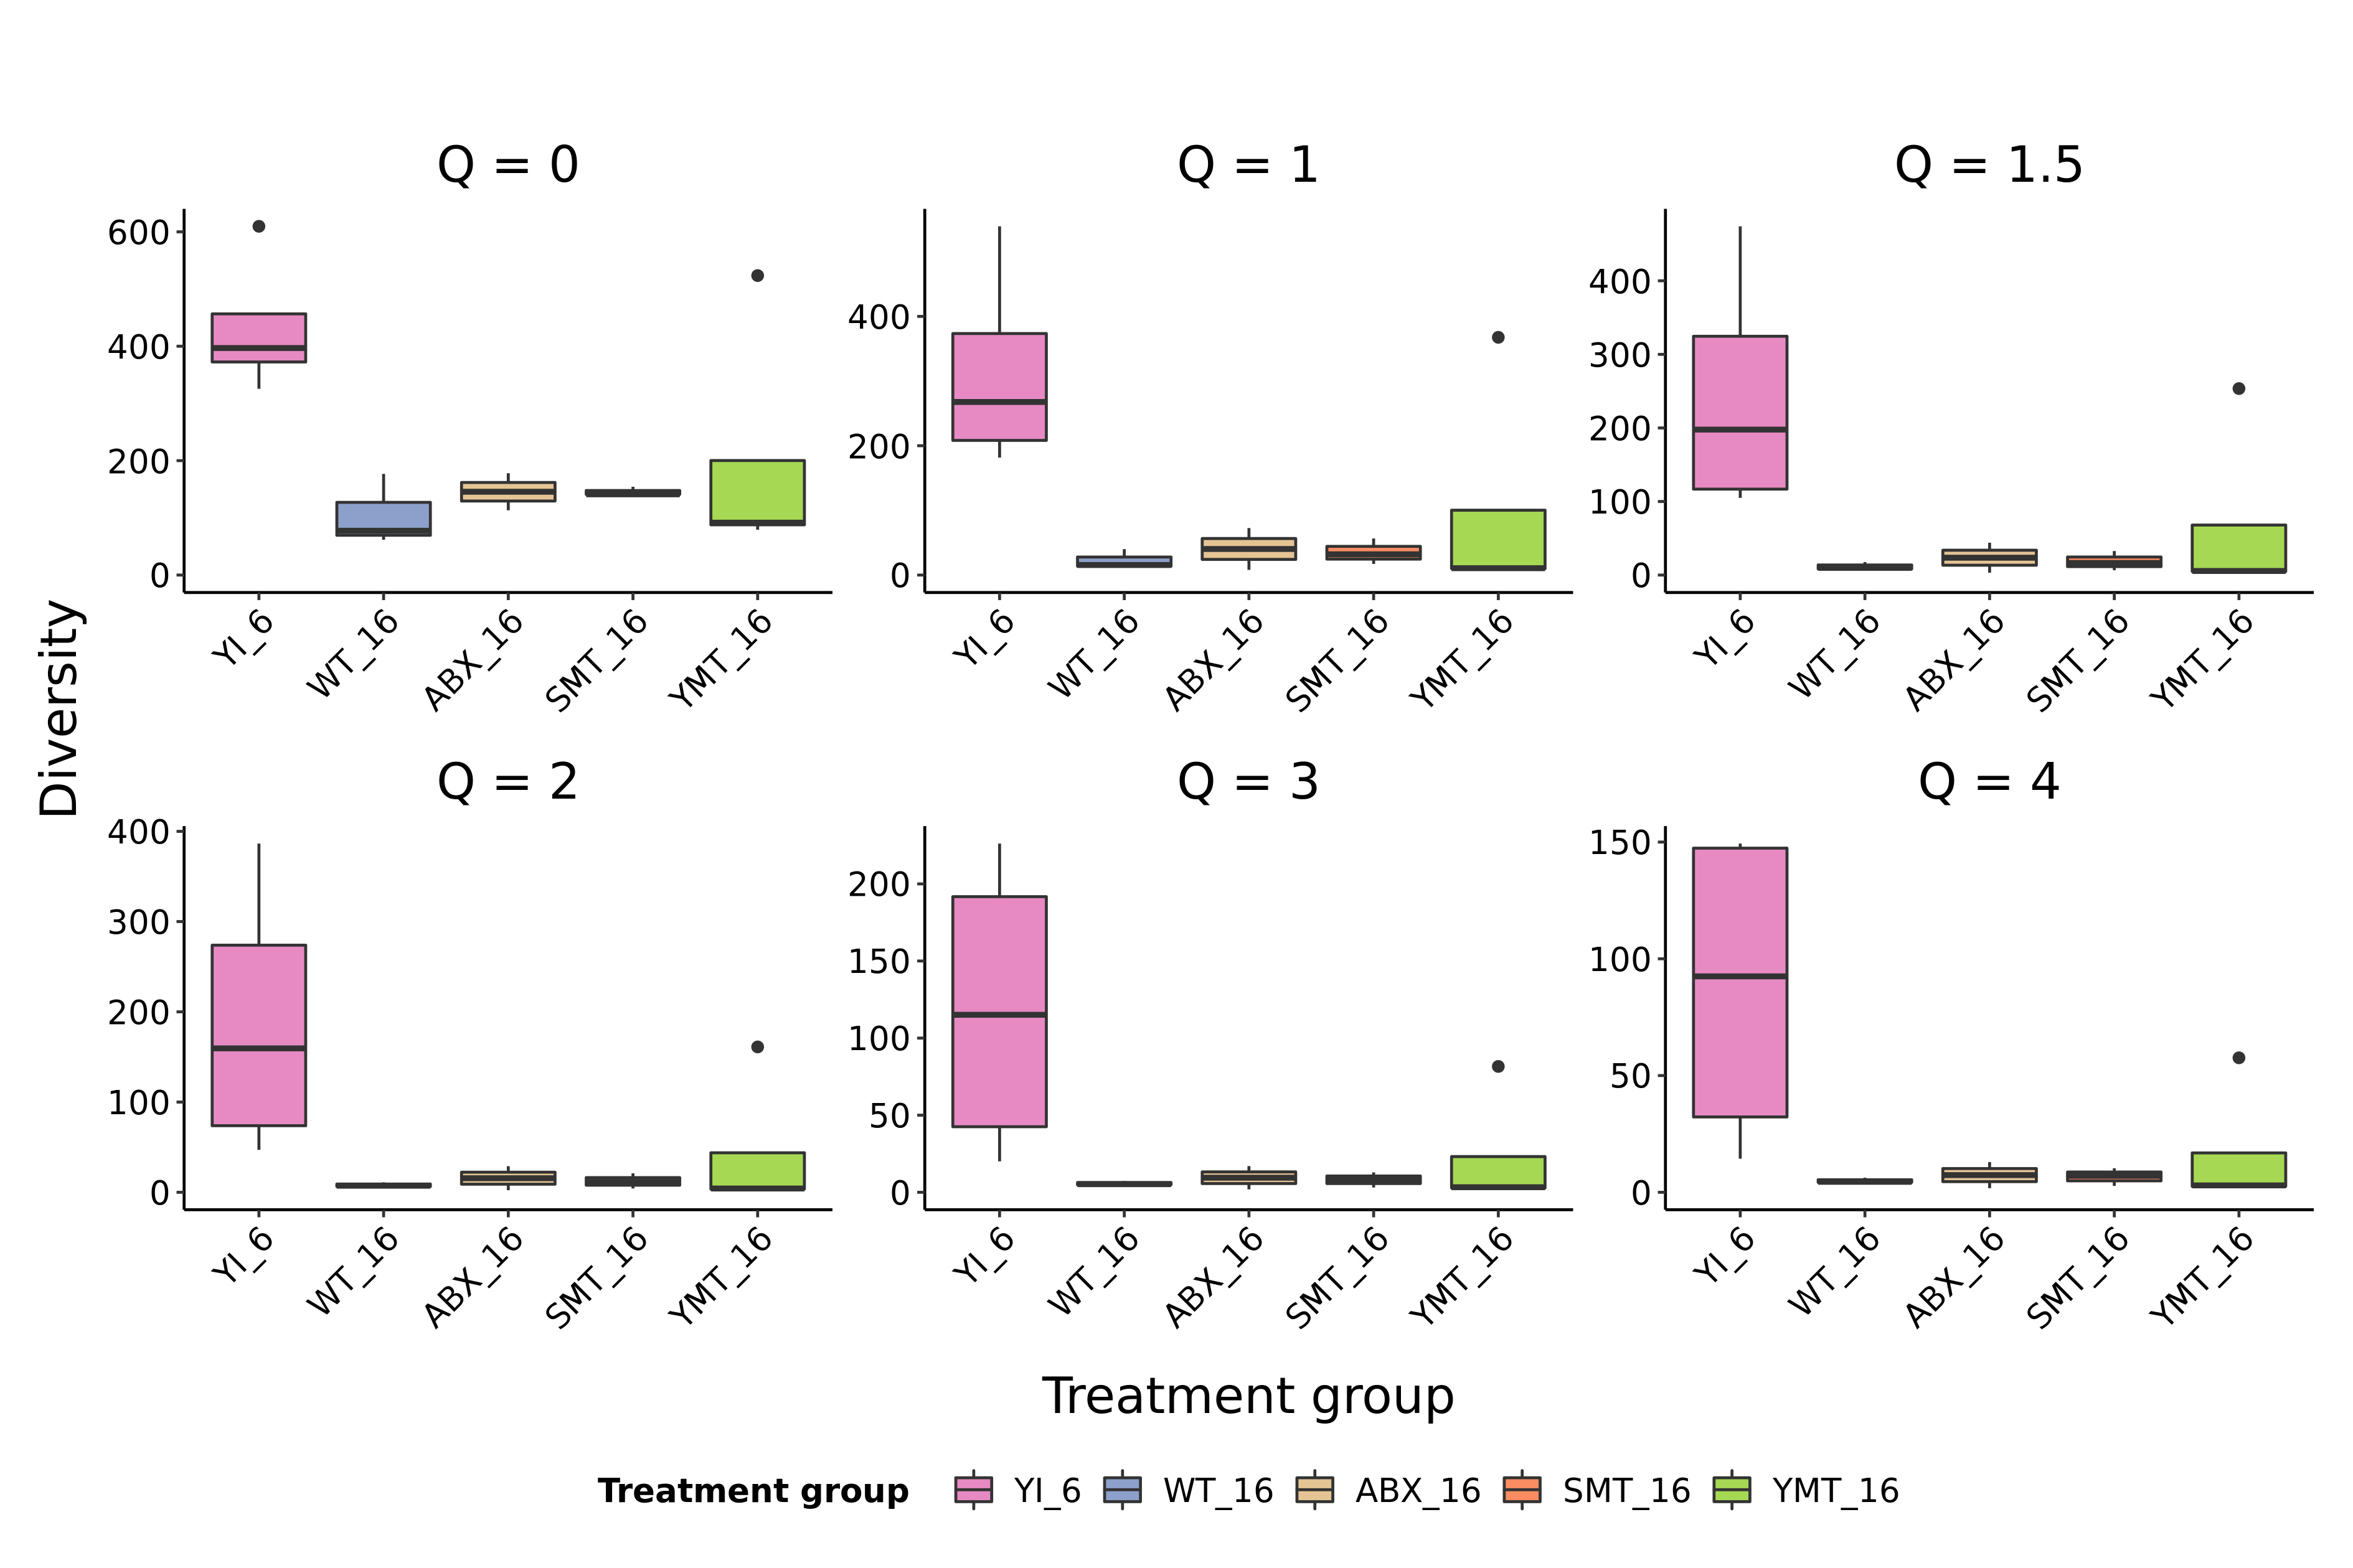
\includegraphics[width = 0.9\textwidth]{_Figures/png/igseq-gut-clone-diversity-solo-groups}
\caption[Comparing clonal alpha-diversities between treatment groups in the \igseq gut dataset]{\textbf{Comparing clonal alpha-diversities between treatment groups in the \igseq gut dataset:} Boxplots of clonal Hill diversity values for the antibody repertoires of individuals of each treatment group in the \igseq gut dataset at a sample of diversity orders. Pairwise $p$-values are computed using nonparametric Mann–Whitney U tests ($*: 0.01 < p \leq 0.05;~**: 0.001 < p \leq 0.01;~***: p \leq 0.001$).}
\label{fig:igseq-gut-clone-diversity-solo-groups}
\end{figure}

\begin{figure}
\centering
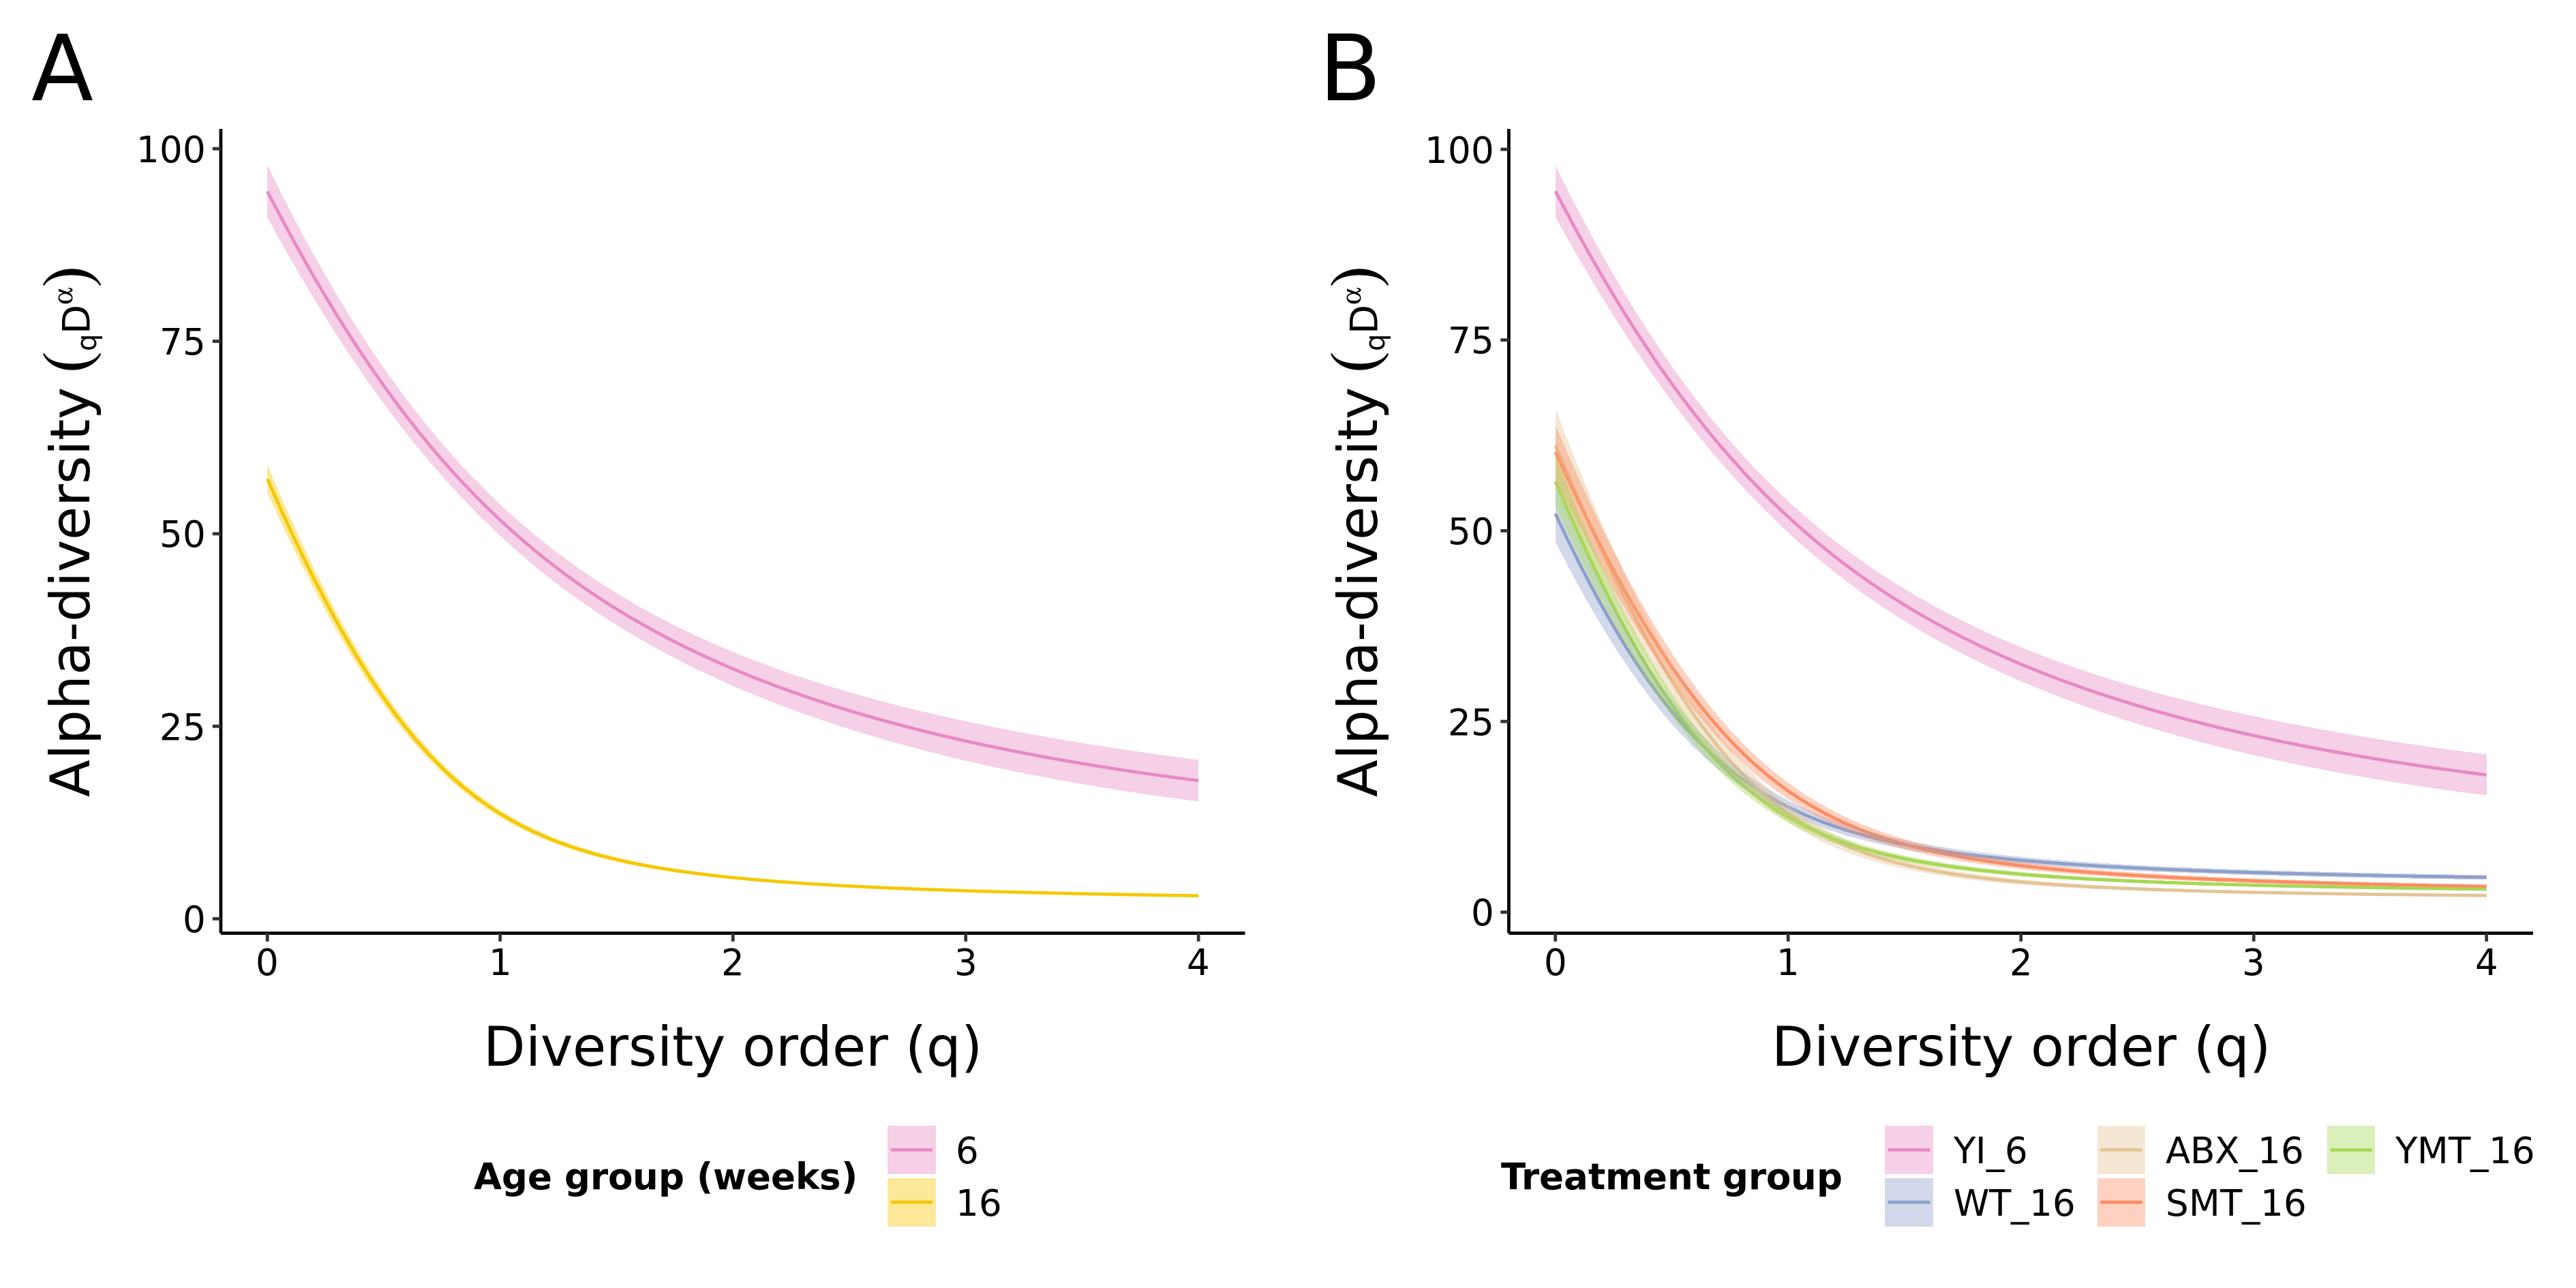
\includegraphics[width = 0.9\textwidth]{_Figures/png/igseq-gut-VJ-diversity-alpha}
\begin{subfigure}{0em}
\phantomsubcaption{}
\label{fig:igseq-gut-VJ-diversity-alpha-age}
\end{subfigure}
\begin{subfigure}{0em}
\phantomsubcaption{}
\label{fig:igseq-gut-VJ-diversity-alpha-groups}
\end{subfigure}
\caption[VJ alpha-diversity spectra for \igseq gut dataset]{\textbf{VJ alpha-diversity spectra for \igseq gut dataset:} Bootstrapped alpha-diversity spectra of VJ usage for each (A) age group and (B) treatment group in the \igseq ageing dataset, as measured by number of unique sequences per unambiguous VJ identity. Shaded regions in both subfigures represent 95\,\% confidence intervals, estimated using bootstrapping.}
\label{fig:igseq-gut-VJ-diversity-alpha}
\end{figure}

\begin{figure}
\centering
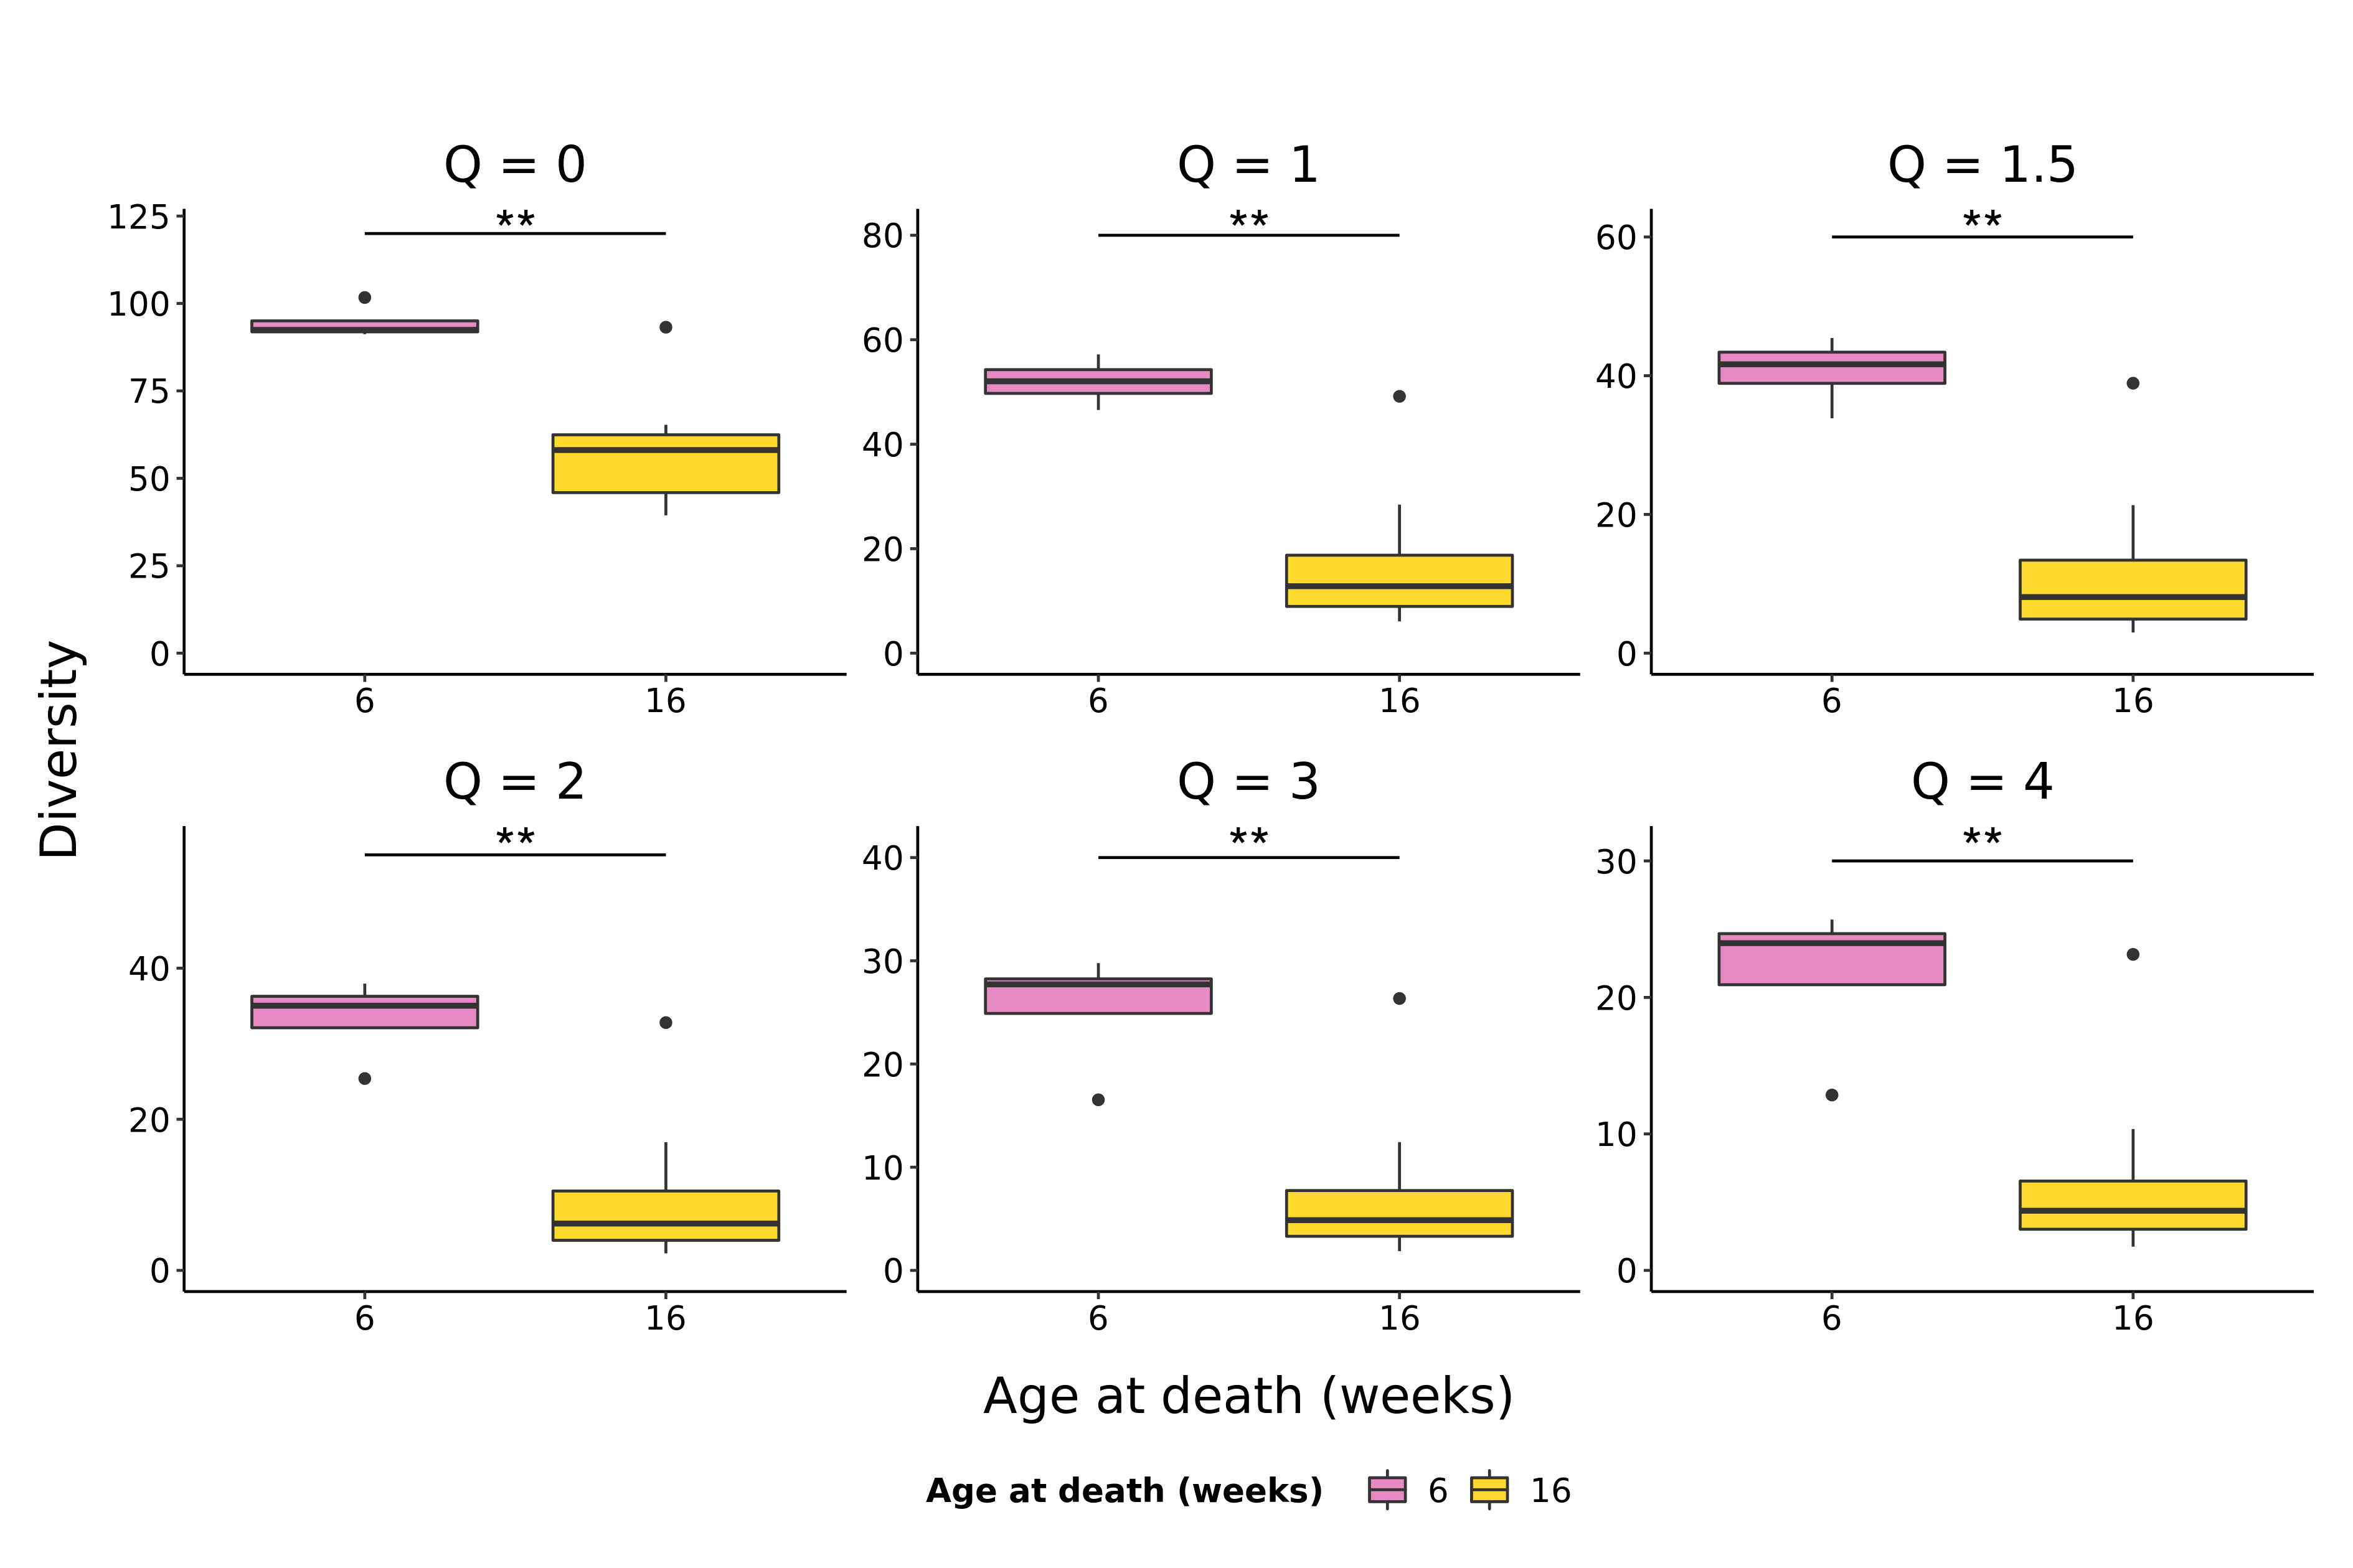
\includegraphics[width = 0.9\textwidth]{_Figures/png/igseq-gut-VJ-diversity-solo-age}
\caption[Comparing VJ alpha-diversities between age groups in the \igseq gut dataset]{\textbf{Comparing VJ alpha-diversities between age groups in the \igseq gut dataset:}Boxplots of VJ Hill diversity values for the antibody repertoires of individuals of each age group in the \igseq gut dataset at a sample of diversity orders. Pairwise $p$-values are computed using nonparametric Mann–Whitney U tests ($*: 0.01 < p \leq 0.05;~**: 0.001 < p \leq 0.01;~***: p \leq 0.001$).}
\label{fig:igseq-gut-VJ-diversity-solo-age}
\end{figure}

\begin{figure}
\centering
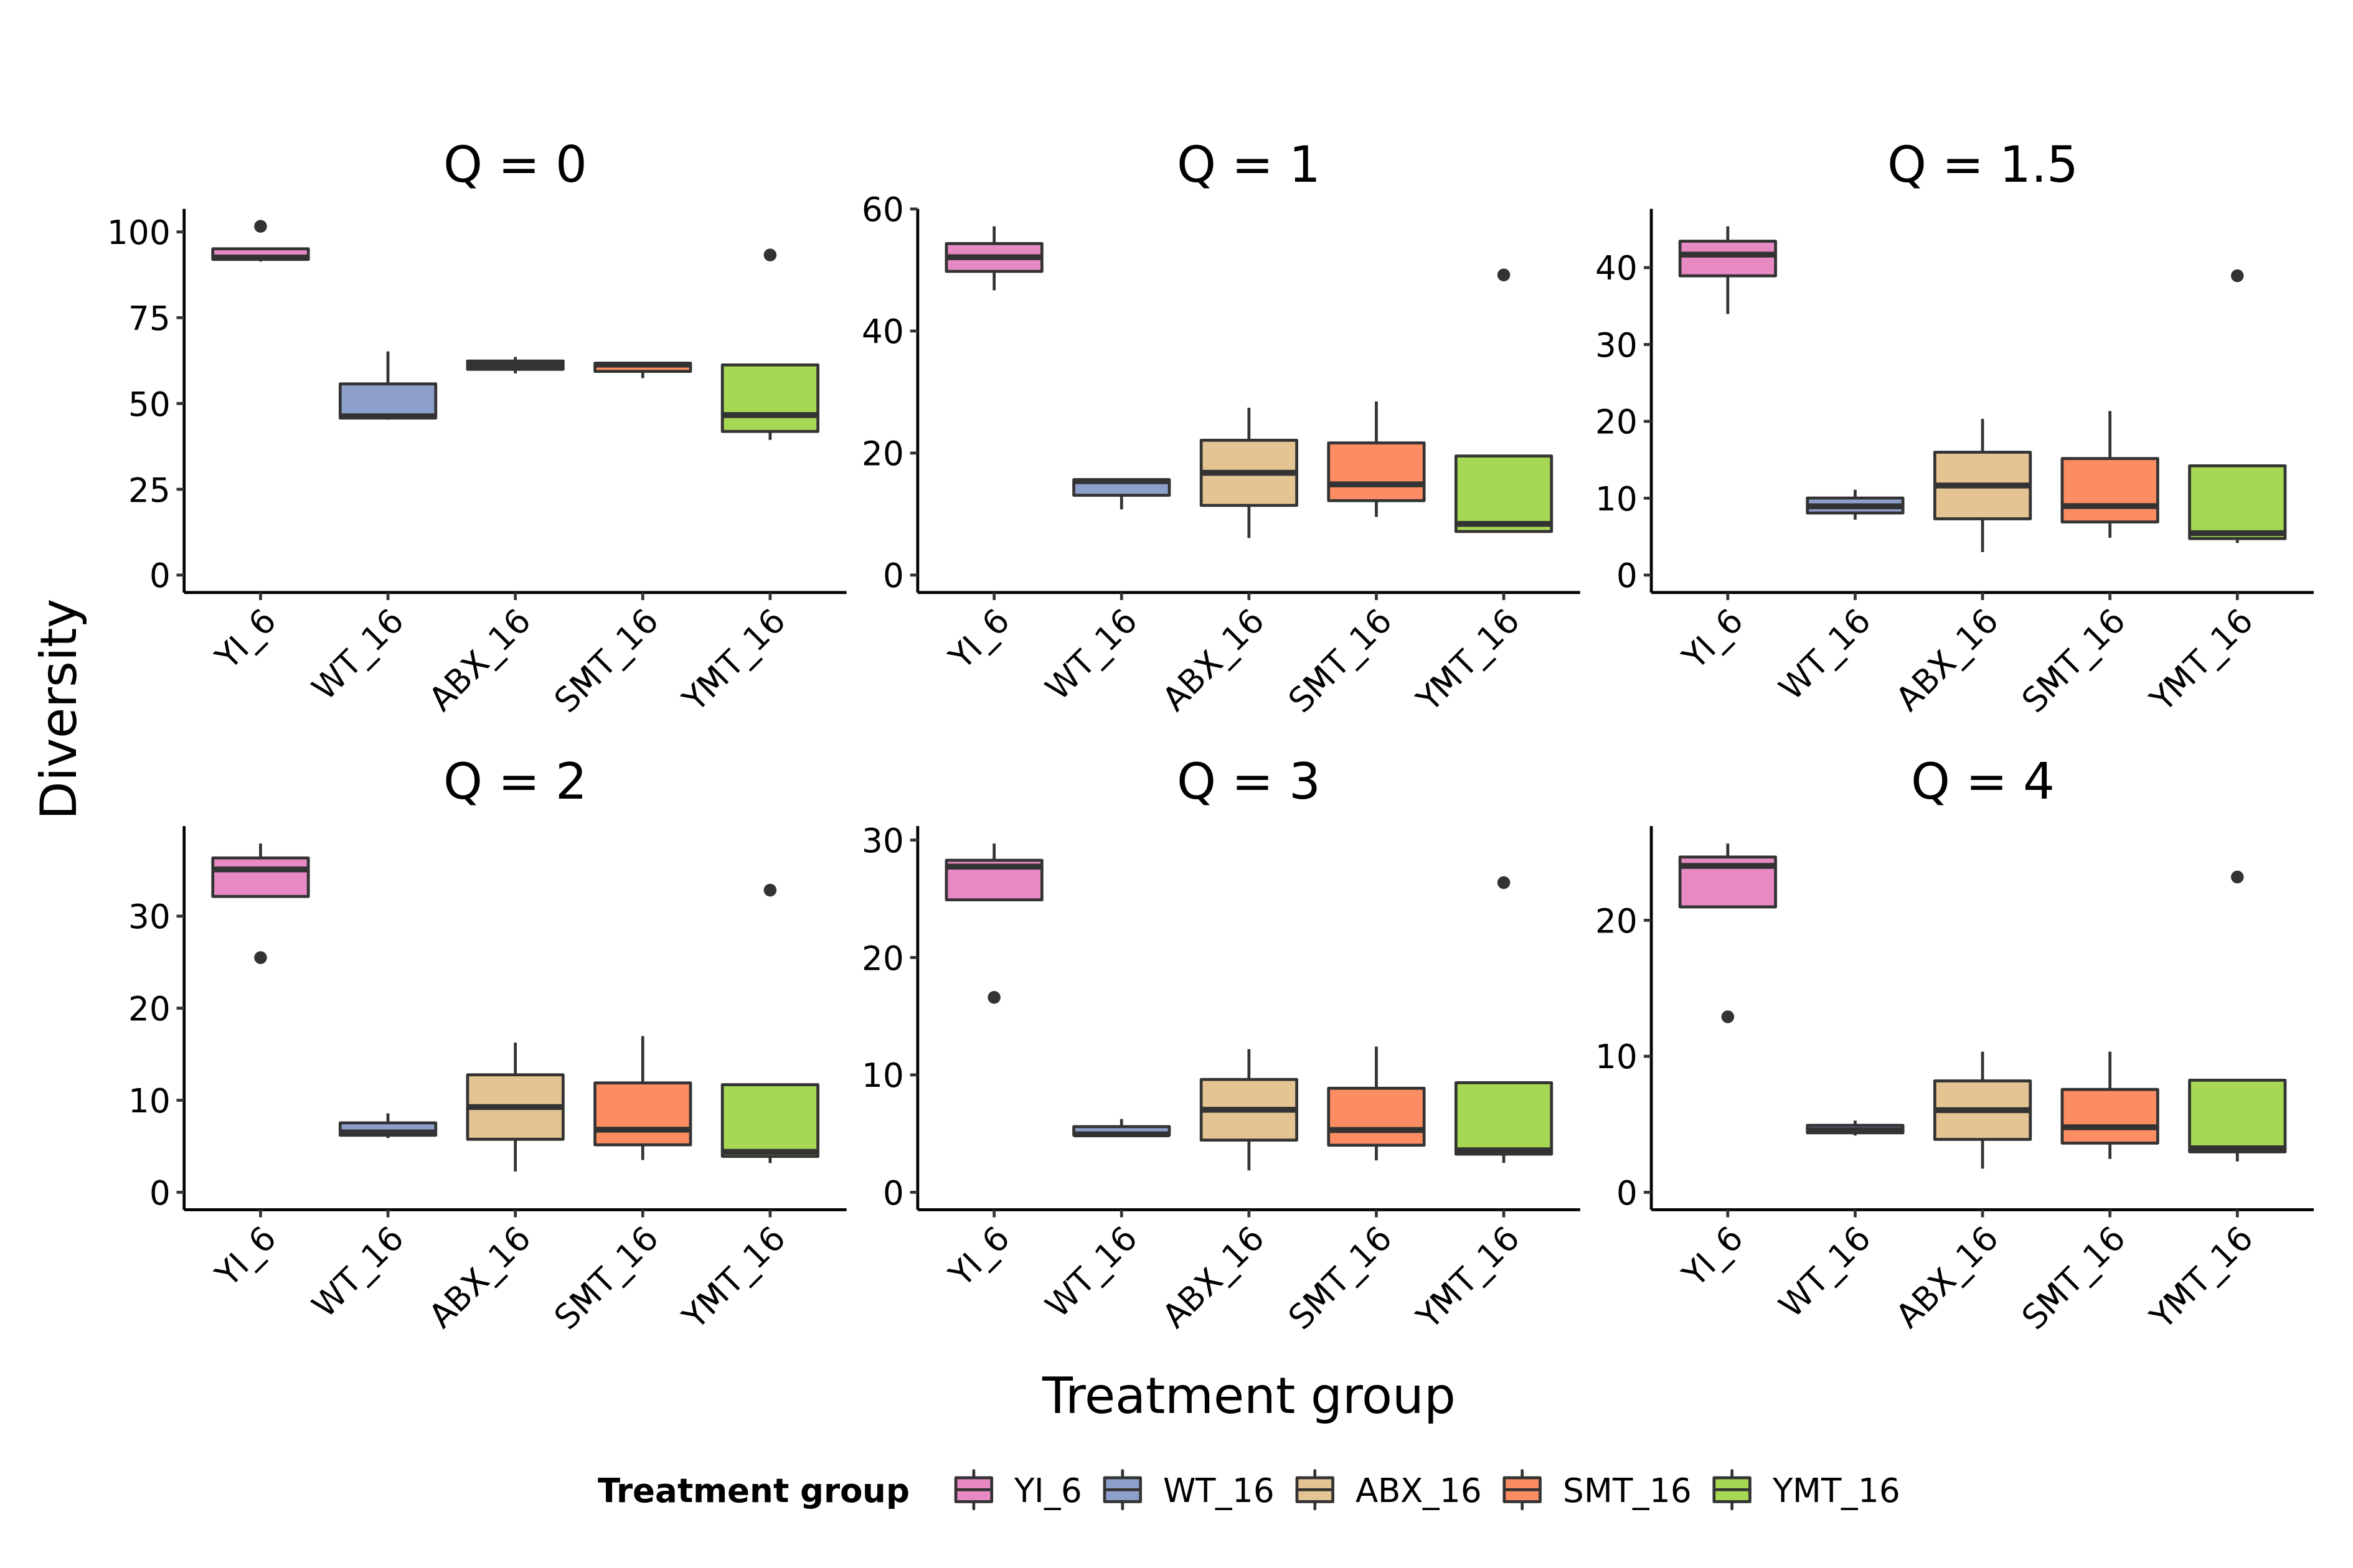
\includegraphics[width = 0.9\textwidth]{_Figures/png/igseq-gut-VJ-diversity-solo-groups}
\caption[Comparing VJ alpha-diversities between treatment groups in the \igseq gut dataset]{\textbf{Comparing VJ alpha-diversities between treatment groups in the \igseq gut dataset:} Boxplots of VJ Hill diversity values for the antibody repertoires of individuals of each treatment group in the \igseq gut dataset at a sample of diversity orders. Pairwise $p$-values are computed using nonparametric Mann–Whitney U tests ($*: 0.01 < p \leq 0.05;~**: 0.001 < p \leq 0.01;~***: p \leq 0.001$).}
\label{fig:igseq-gut-VJ-diversity-solo-groups}
\end{figure}

In terms of beta-diversity, the Hill-spectrum results (\Cref{fig:igseq-gut-VJ-diversity-beta}) are equivocal, with large differences in diversity between age groups observed at intermediate diversity orders (c. 1 to 2.5) but not at very low or very high orders (\Cref{fig:igseq-gut-VJ-diversity-beta-age}). Different treatment groups, meanwhile, exhibit very different patterns of beta diversity at higher orders (\Cref{fig:igseq-gut-VJ-diversity-beta-groups}), but not in any clear pattern: the antibiotic-treated and same-age-transfer groups show very high high-order beta diversity, indicating nearly maximal difference between individuals in their VJ-usage profiles, while the untreated and same-age-transfer groups show much lower between-individual variablity. To more closely investigate differences in inter-individual variability between sample groups, I again computed repertoire dissimilarity index (RDI) distances between each pair of individual repertoires in the dataset, and visualised the results by age cohort (\Cref{fig:igseq-gut-rdi-VJ-individual-age}) and treatment group (\Cref{fig:igseq-gut-rdi-VJ-individual-group}). The results again indicate large differences in VJ-usage variability between young and old gut repertoires in the turquoise killifish, with young samples clustering much more closely together (\Cref{fig:igseq-gut-rdi-VJ-individual-age-pcoa-facet}) and exhibiting consequently much lower pairwise RDI distances (\Cref{fig:igseq-gut-rdi-VJ-individual-age-groupdist-all,fig:igseq-gut-rdi-VJ-individual-age-groupdist-nn}); conversely, there is no significant difference in RDI distribution between the different 16-week-old treatment groups, indicating that the different groups are similar in their inter-individual variability. These RDI results contrast markedly with the differences in beta-spectra observed in \Cref{fig:igseq-gut-VJ-diversity-beta-groups}, suggesting that the latter may not be reliable measures of significant differences in intra-group variablity when sample sizes are small.

\begin{figure}
\centering
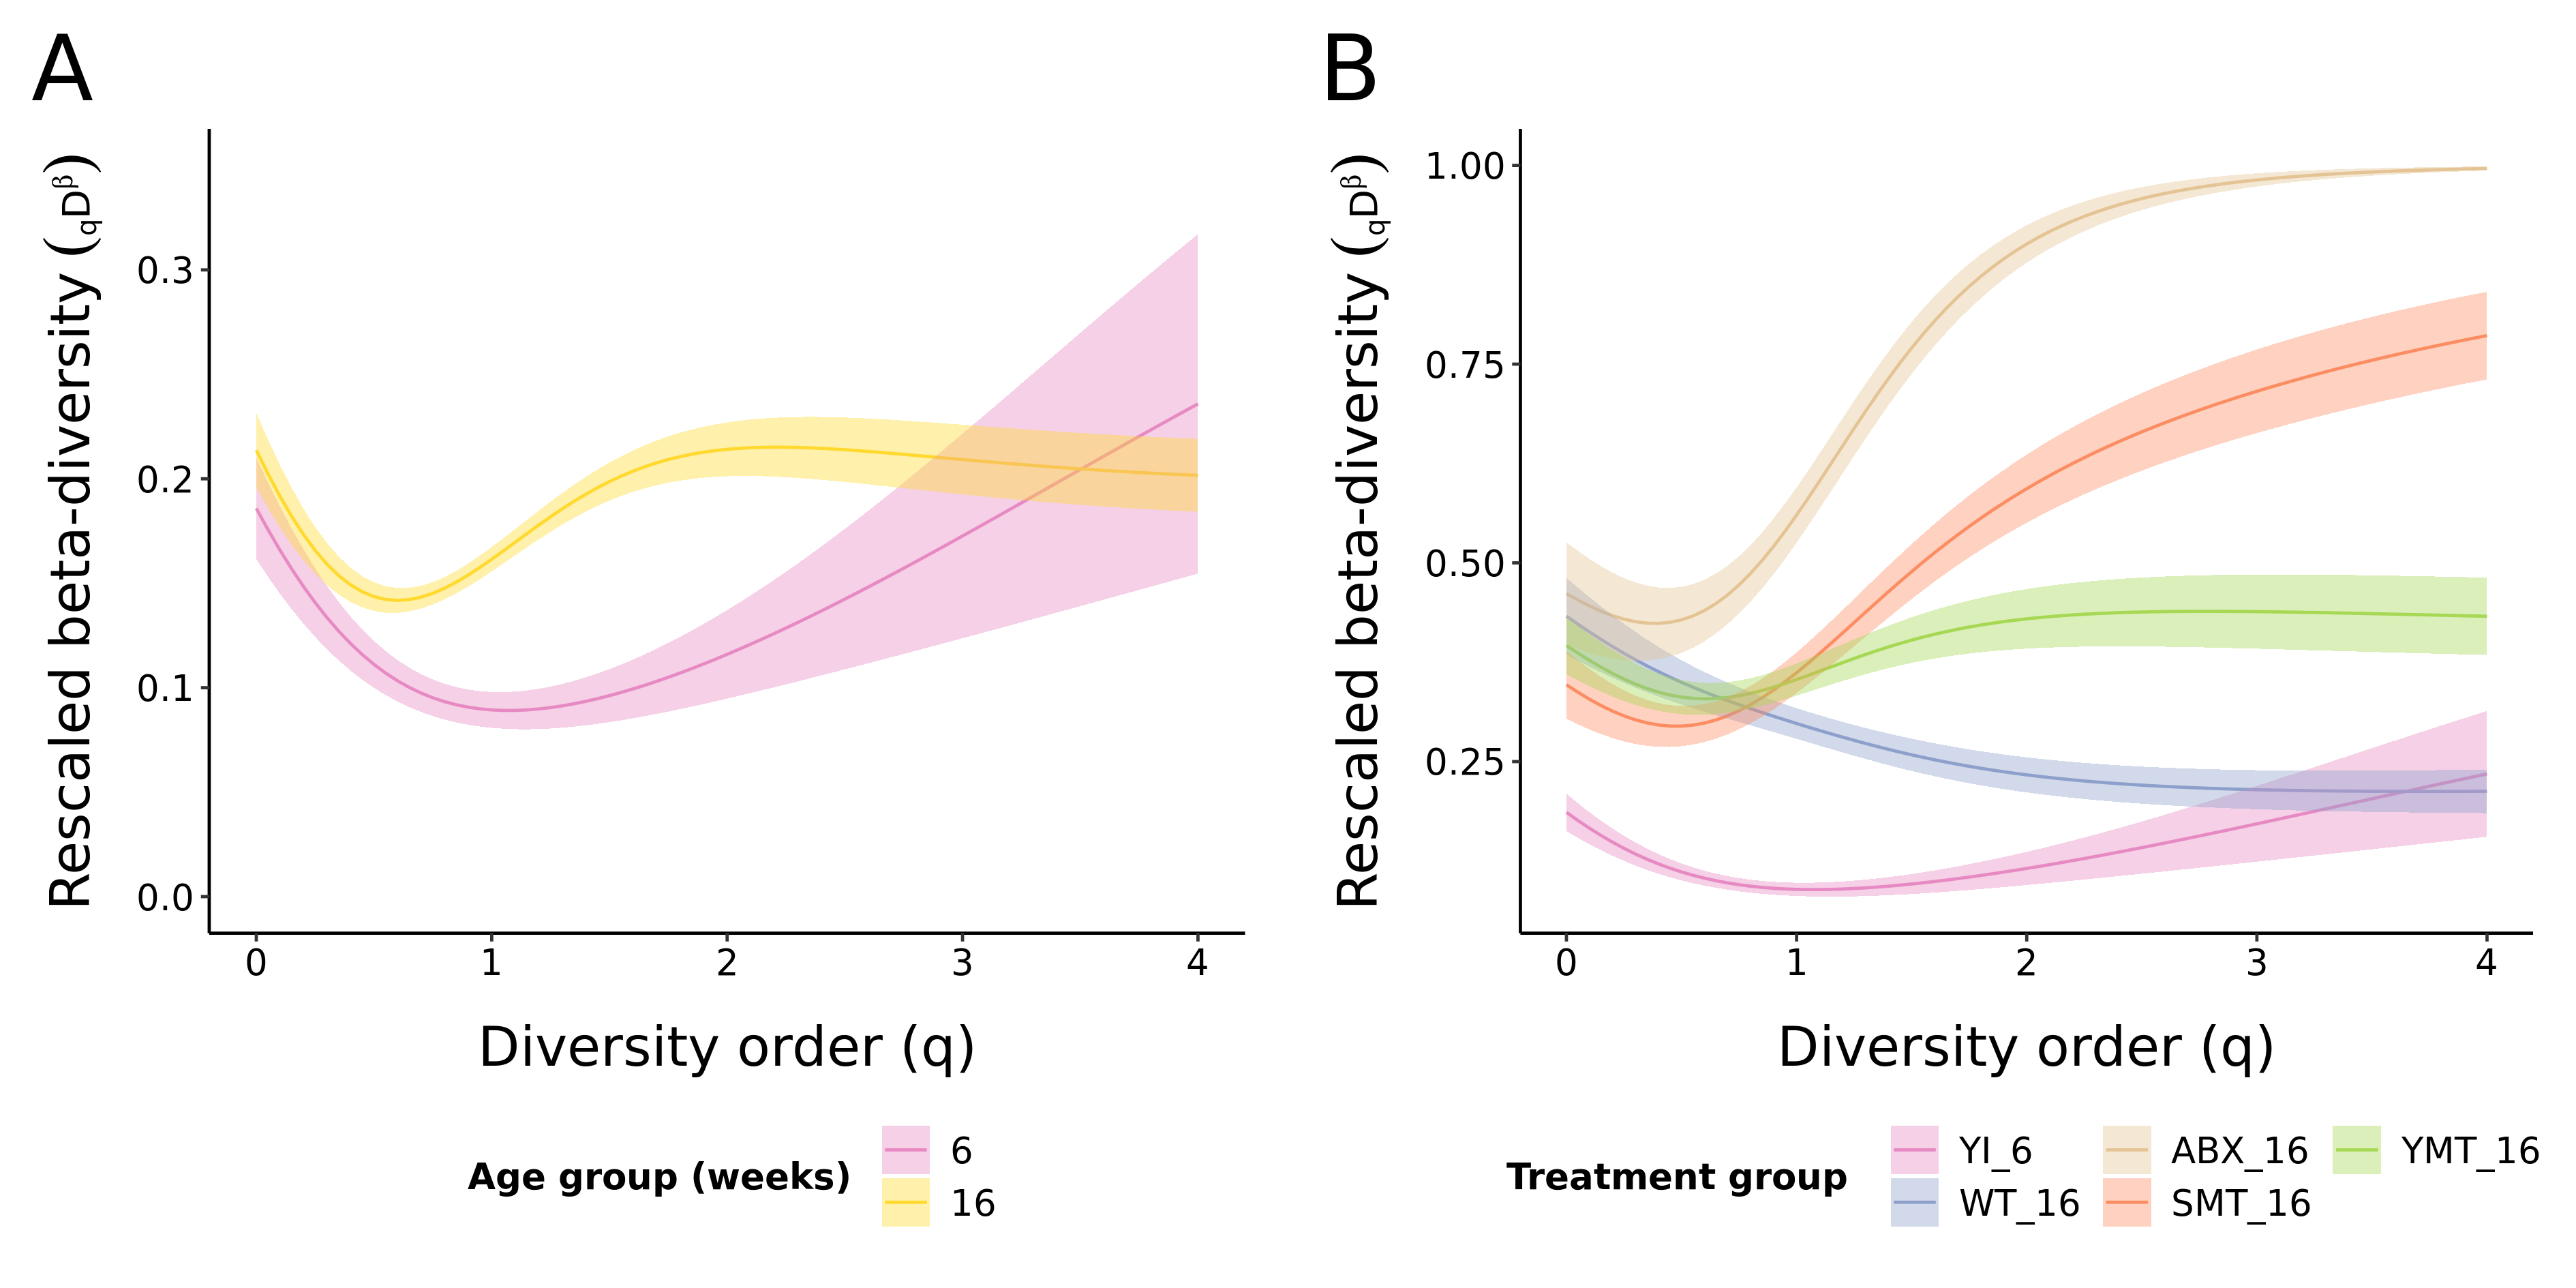
\includegraphics[width = 0.9\textwidth]{_Figures/png/igseq-gut-VJ-diversity-beta}
\begin{subfigure}{0em}
\phantomsubcaption{}
\label{fig:igseq-gut-VJ-diversity-beta-age}
\end{subfigure}
\begin{subfigure}{0em}
\phantomsubcaption{}
\label{fig:igseq-gut-VJ-diversity-beta-groups}
\end{subfigure}
\caption[VJ beta-diversity spectra for \igseq gut dataset]{\textbf{VJ beta-diversity spectra for \igseq gut dataset:} Bootstrapped beta-diversity spectra of VJ usage for each (A) age group and (B) treatment group in the \igseq ageing dataset, as measured by number of unique sequences per unambiguous VJ identity. Shaded regions in both subfigures represent 95\,\% confidence intervals, estimated using bootstrapping.}
\label{fig:igseq-gut-VJ-diversity-beta}
\end{figure}

\begin{figure}
\centering
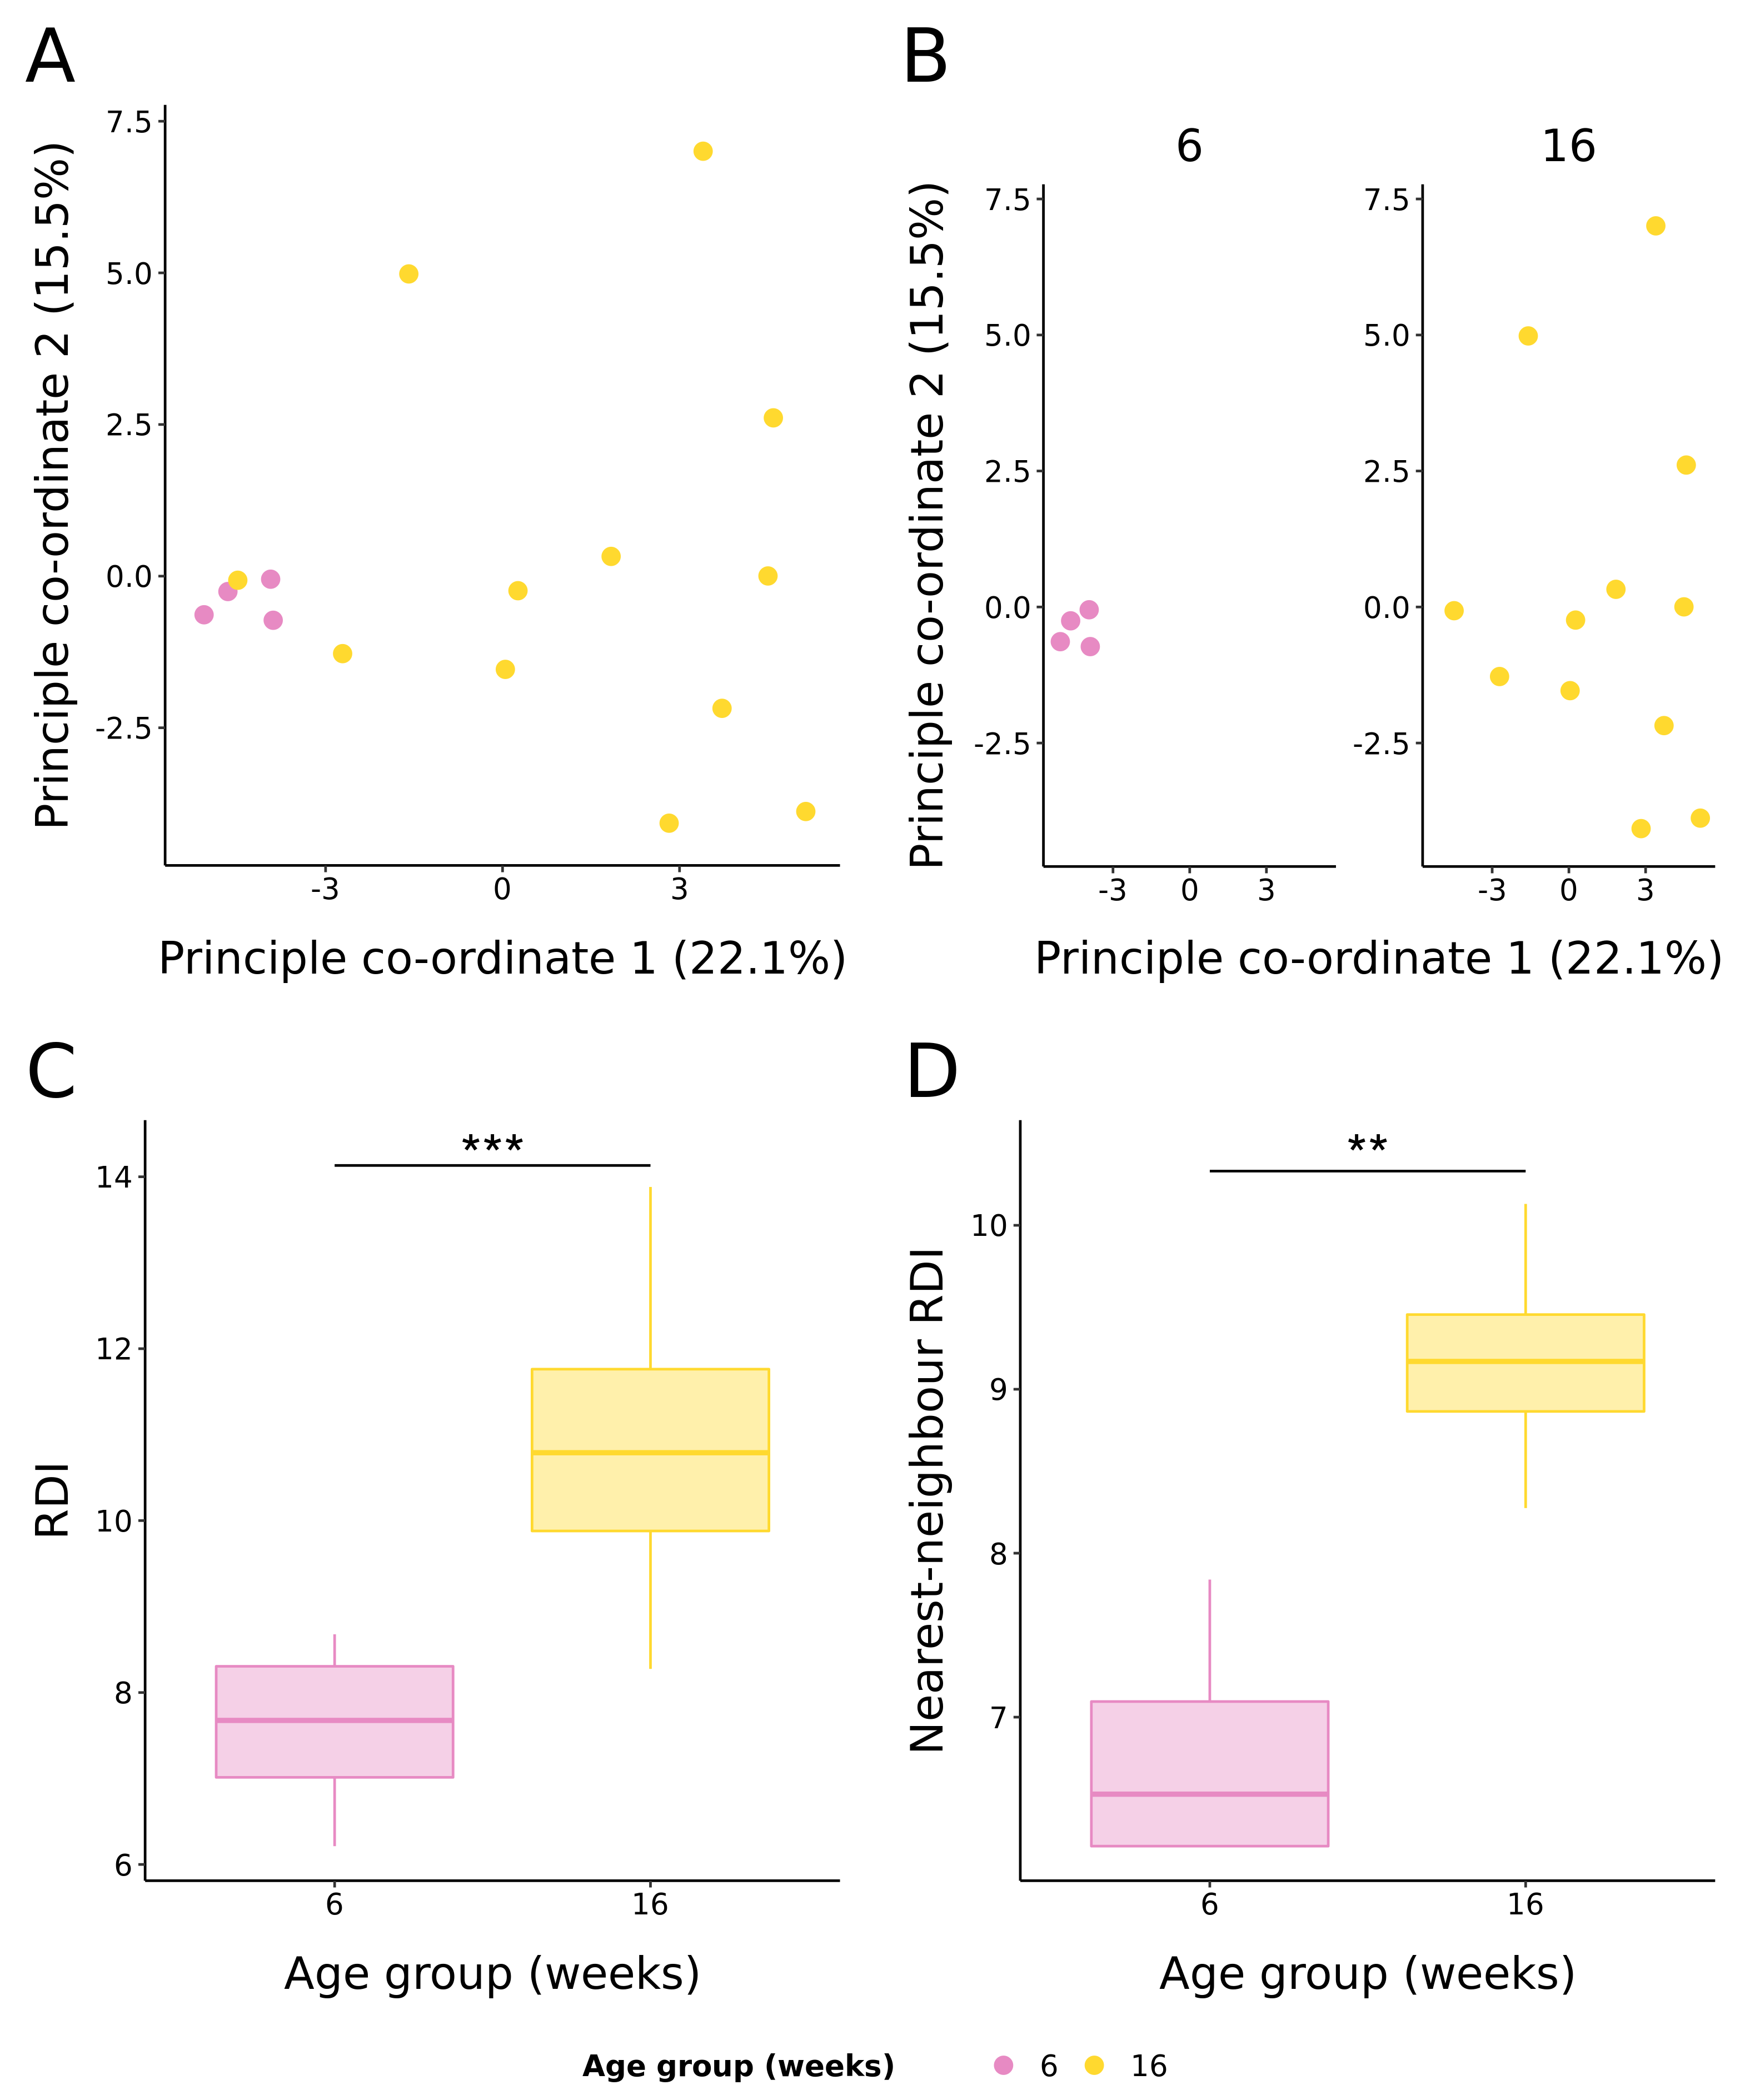
\includegraphics[width = 0.9\textwidth]{_Figures/png/igseq-gut-rdi-VJ-individual-age}
\begin{subfigure}{0em}
\phantomsubcaption{}
\label{fig:igseq-gut-rdi-VJ-individual-age-pcoa-all}
\end{subfigure}
\begin{subfigure}{0em}
\phantomsubcaption{}
\label{fig:igseq-gut-rdi-VJ-individual-age-pcoa-facet}
\end{subfigure}
\begin{subfigure}{0em}
\phantomsubcaption{}
\label{fig:igseq-gut-rdi-VJ-individual-age-groupdist-all}
\end{subfigure}
\begin{subfigure}{0em}
\phantomsubcaption{}
\label{fig:igseq-gut-rdi-VJ-individual-age-groupdist-nn}
\end{subfigure}
\caption[Intra-age-group variability in VJ expression in the \igseq gut dataset]{\textbf{Intra-age-group variability in VJ expression in the \igseq gut dataset:} (A-B) Principal co-ordinate analysis (PCoA) of pairwise inter-individual VJ-RDI distances, coloured by age group and displayed together (A) or separately by age group (B). (C-D) Boxplots of overall (C) and nearest-neighbour (D) inter-individual VJ-RDI distances for each age group in the dataset. Pairwise $p$-values are computed using nonparametric Mann–Whitney U tests ($*: 0.01 < p \leq 0.05;~**: 0.001 < p \leq 0.01;~***: p \leq 0.001$).}
\label{fig:igseq-gut-rdi-VJ-individual-age}
\end{figure}

\begin{figure}
\centering
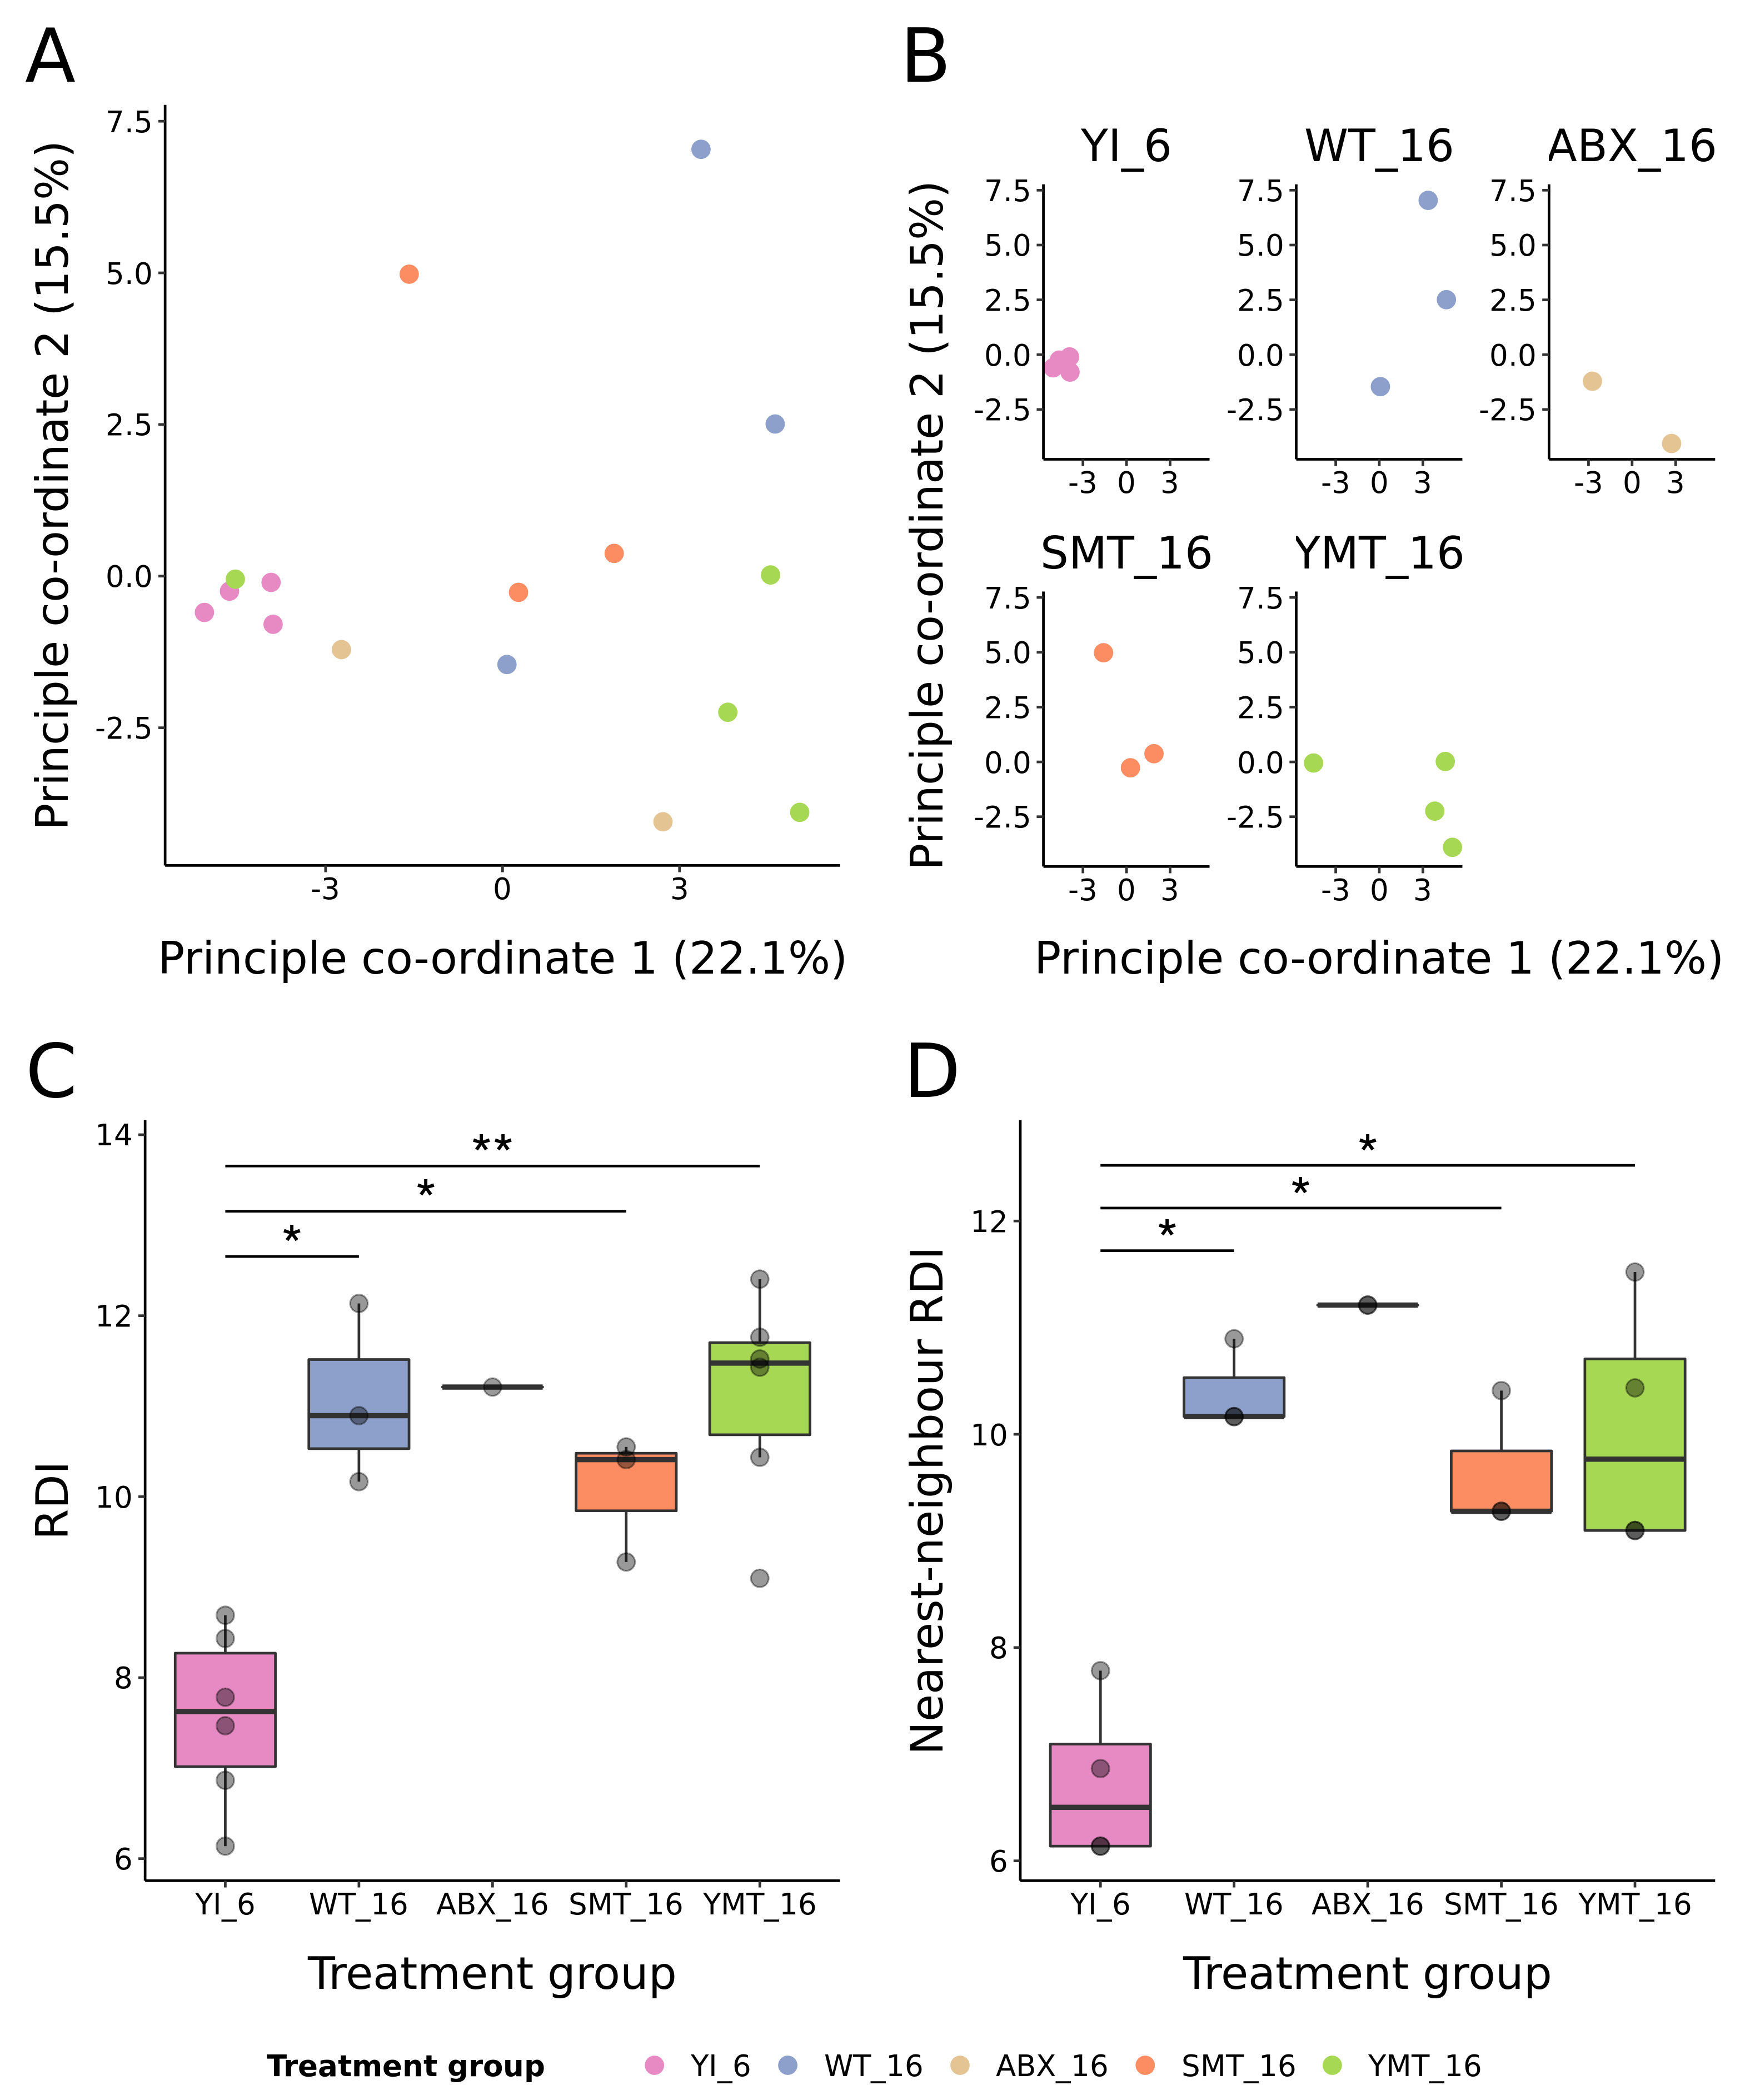
\includegraphics[width = 0.9\textwidth]{_Figures/png/igseq-gut-rdi-VJ-individual-group}
\begin{subfigure}{0em}
\phantomsubcaption{}
\label{fig:igseq-gut-rdi-VJ-individual-group-pcoa-all}
\end{subfigure}
\begin{subfigure}{0em}
\phantomsubcaption{}
\label{fig:igseq-gut-rdi-VJ-individual-group-pcoa-facet}
\end{subfigure}
\begin{subfigure}{0em}
\phantomsubcaption{}
\label{fig:igseq-gut-rdi-VJ-individual-group-groupdist-all}
\end{subfigure}
\begin{subfigure}{0em}
\phantomsubcaption{}
\label{fig:igseq-gut-rdi-VJ-individual-group-groupdist-nn}
\end{subfigure}
\caption[Intra-treatment-group variability in VJ expression in the \igseq gut dataset]{\textbf{Intra-treatment-group variability in VJ expression in the \igseq gut dataset:} (A-B) Principal co-ordinate analysis (PCoA) of pairwise inter-individual VJ-RDI distances, coloured by treatment group and displayed together (A) or separately by treatment group (B). (C-D) Boxplots of overall (C) and nearest-neighbour (D) inter-individual VJ-RDI distances for each treatment group in the dataset. Pairwise $p$-values are computed using nonparametric Mann–Whitney U tests ($*: 0.01 < p \leq 0.05;~**: 0.001 < p \leq 0.01;~***: p \leq 0.001$).}
\label{fig:igseq-gut-rdi-VJ-individual-group}
\end{figure}

In terms of repertoire ageing, therefore, the gut repertoire not only reproduces the whole-body phenotype of reduced alpha- and increased beta-diversity with age, but in fact shows an stronger ageing phenotype than the whole-body repertoires reported in \Cref{sec:igseq_ageing}. In addition to showing a much stronger age-related decline in clonal alpha-diversity with age than that exhibited in the ageing dataset (\Cref{fig:igseq-ageing-clone-diversity-alpha,fig:igseq-ageing-clone-diversity-solo-fit-gamma}), the gut repertoire also shows a strong age-related decline in VJ alpha-diversity, something not observed in the whole-body data (\Cref{fig:igseq-ageing-VJ-diversity-alpha,fig:igseq-ageing-VJ-diversity-solo-fit-gamma}). This latter difference is likely due to the much lower clonal richness and higher oligoclonality exhibited by the gut repertoires (\Cref{fig:igseq-rarefied-clone-counts,fig:igseq-rarefied-clone-p20,fig:igseq-rarefied-clone-counts-size}): when the local repertoire contains fewer small \naive clones and exhibits a greater degree of domination by the few largest clones, differences in VJ-usage between these large, activated clones may outweigh (presumably similar) VJ-usage distributions in small, \naive clones to a greater extent than in the much-more-polyclonal whole-body repertoire. The much stronger loss in clonal diversity in gut repertoires, meanwhile, may be attributable to the especially-strong antigenic challenge at the mucosal surface, resulting in high levels of clonal expansion and progressive domination of the mucosal B-cell niche by a small number of highly expanded clones \parencite{caruso2009immunosenescence}; this phenomenon could in turn be exacerbated by the observed loss of phenotypic diversity (but not total abundance) in the gut microbiota \parencite{smith2017microbiota}, which might progressively reduce the variety of antigenic exposure at the mucosal surface and so further encourage a restriction in clonal diversity. If so, the strength of the ageing phenotype in these repertoires may have important consequences for the ability of the organism to regulate its mucosal microbiotal environment. More research is needed, however, to determine the mechanisms, kinetics and importance of mucosal repertoire ageing in turquoise killifish.

In sharp contrast to the age-related changes observed in the gut antibody repertoire, there is no strong evidence from these analyses supporting the hypothesis that gut-microbiota transfer from young fish rejuvenates the antibody repertoire. While the alpha-diversity spectrum of the YMT group appears to be slightly higher than the OMT/ABX groups at very low diversity orders (\Cref{fig:igseq-gut-clone-diversity-alpha-groups}), these indications are not borne out by subsequent statistical analysis, and it is precisely these low-order diversity metrics that are most vulnerable to sampling bias and undersampling (a pervasive problem in immune-repertoire sequencing \parencite{mora2016diversity}). There is also no obvious difference in VJ alpha-diversity between treatment groups, while the beta-diversity of the YMT group is non-significantly \textit{higher} than that of the untreated control group (\Cref{fig:igseq-gut-VJ-diversity-beta-groups,fig:igseq-gut-rdi-VJ-individual-group-groupdist-all}). Overall, whatever mechanism underlies the effect of gut microbiota transfer on killifish lifespan \parencite{smith2017microbiota}, it does not appear to be operating through modulation of gut antibody-repertoire diversity.